\documentclass{article}
\usepackage{graphicx}
\usepackage{hyperref}
\usepackage{amsmath}
\usepackage{geometry}
\usepackage{booktabs}
\usepackage[toc,page]{appendix}
\usepackage{tikz}
\usetikzlibrary{arrows.meta,shapes.geometric}
\geometry{a4paper, margin=2.5cm}

\title{Non-Shot Expected Goals: A Progressive Machine Learning Approach to Modelling Attacking Threat in Football}
\author{Adam Marshall}
\date{January 2026}

\begin{document}

\maketitle

% ============================================================
% ABSTRACT
% ============================================================
% TODO: Write ~200 words covering:
%   - The problem: traditional xG models evaluate shots only, ignoring ~95% of play
%   - Your approach: three progressive architectures (Random Forest → CNN → Transformer)
%   - Data: StatsBomb open data (3,464 matches / 6.1M events) + 360 freeze-frame (323 matches)
%   - Key results: v1 ROC AUC 0.6828, v2 ROC AUC 0.8416 (+16pp), v3 ROC AUC 0.8459 (+0.4pp over v2)
%   - Conclusion: standardised evaluation framework shows clear, measurable progression
\begin{abstract}
Expected Goals (xG) is the dominant metric in modern football analytics, but it evaluates shots only, accounting for fewer than 2\% of all possession events. The remaining 98\%, comprising every pass, carry, and dribble that builds towards a scoring opportunity, carry no quantified threat value under the standard framework.

This project develops a Non-Shot Expected Threat (xT) model that assigns a goal probability to every on-ball event in a match, progressing through three increasingly sophisticated architectures. Version 1 uses a Random Forest trained on ten scalar features covering ball position, distance and angle to goal, action type, match period, elapsed minute, running score differential, and team form, extracted from the full StatsBomb open dataset (3,464 matches, 6.1 million events), achieving a test ROC AUC of 0.6828. Version 2 replaces this with a dual-branch Convolutional Neural Network that encodes the pitch as a six-channel spatial image using StatsBomb 360 freeze-frame data, incorporating the positions of all 22 players; this raises test ROC AUC to 0.8416. Version 3 adds a Transformer-based cross-attention layer on top of the frozen Version 2 CNN, treating each player as an individual token to enable explicit relational reasoning about defensive formations; test ROC AUC reaches 0.8459.

A standardised evaluation framework across all three versions (using ROC AUC, Brier Score, Log Loss, and Spearman rank correlation) makes the progression directly legible. An interactive Flask-based frontend accompanies Version 3, allowing users to place players on a virtual pitch and explore predicted threat values in real time.
\end{abstract}

\newpage
\tableofcontents
\newpage

% ============================================================
\section*{Acknowledgements}
% ============================================================
% TODO: Brief acknowledgements — typically 1 short paragraph.
% Suggested content: thank your supervisor, acknowledge StatsBomb for making
% their open data freely available for research, and note the GPU resource used.
I would like to thank my supervisors, Dr Ioanna Papatsouma and Sam Brzezicki, for their guidance and support throughout this project. I am grateful to StatsBomb for making their event data and 360 freeze-frame data freely available for academic and non-commercial use (\url{https://github.com/statsbomb/open-data}). Model training was carried out on an NVIDIA RTX 6000 Ada GPU.

\newpage

% ============================================================
\section{Introduction}
% ============================================================

Expected Goals (xG) is a metric widely used in modern football analytics to quantify the quality of scoring chances. Traditional xG models focus exclusively on shots, estimating the probability that a given attempt results in a goal based on factors such as distance, angle, and shot type. However, this approach captures only a small slice of a football match; the vast majority of play consists of passes, carries, and dribbles that build towards a scoring opportunity. A metric that can quantify the threat posed by any moment of possession, not just shots, is therefore far more informative.

This project develops a \textbf{Non-Shot Expected Goals} model (also referred to as Expected Threat, or xT), which assigns a probability to every event in a match (pass, carry, dribble, or shot) reflecting how likely that possession chain is to end in a goal. The project progresses through three increasingly sophisticated model versions:

\begin{enumerate}
    \item \textbf{Version 1}: A Random Forest model trained on ten scalar features (position, angle, distance, action type, period, minute, score differential, and team form) extracted from raw StatsBomb event data.
    \item \textbf{Version 2}: A dual-branch Convolutional Neural Network (CNN) and Multi-Layer Perceptron (MLP), exploiting StatsBomb 360 freeze-frame data to encode the positions of all players on the pitch as spatial image channels.
    \item \textbf{Version 3}: A two-stage architecture that freezes the trained Version 2 CNN and adds a Transformer-based cross-attention layer, allowing the model to explicitly reason about the spatial relationships between players when estimating threat.
\end{enumerate}

A Flask-based interactive web frontend accompanies Version 3, allowing users to place players on a virtual pitch and receive a real-time weighted xT prediction.

% TODO: Add the following two subsections to complete the Introduction:
\subsection{Project Objectives}
% TODO: State 3--5 clear, numbered objectives. For example:
%   1. Develop a baseline xT model using classical ML on positional features.
%   2. Improve on this baseline by incorporating full player positional context via CNNs.
%   3. Further improve by introducing explicit relational reasoning via a Transformer.
%   4. Establish a standardised evaluation framework to quantify improvement between versions.
%   5. Build an accessible interactive tool to demonstrate the model to non-technical users.
\begin{enumerate}
    \item Develop a baseline Non-Shot xT model using a classical machine learning approach on tabular positional and action-type features.
    \item Improve on this baseline by incorporating full player positional context through a deep learning architecture that encodes the pitch as a spatial image.
    \item Further improve the model by introducing explicit relational reasoning over individual player positions using a Transformer-based attention mechanism.
    \item Establish a standardised, shared evaluation framework to measure and compare model quality across all three versions using a consistent set of metrics.
    \item Build an accessible interactive tool that allows users to visualise model predictions and explore how player positioning affects expected threat in real time.
\end{enumerate}

\subsection{Report Structure}
% TODO: One sentence per section explaining what each covers.
% e.g. "Section 2 reviews relevant literature on xG modelling and attention-based architectures..."
The remainder of this report is structured as follows. Section~\ref{sec:litreview} reviews relevant prior work on expected goals, non-shot threat metrics, and the machine learning architectures used in this project. Section~\ref{sec:dataset} describes the StatsBomb open dataset and how it was processed into training data for each model version. Section~\ref{sec:features} defines the input features used across all three versions. Section~\ref{sec:eval} describes the evaluation framework, the four metrics used, and the design decisions that make cross-version comparisons valid. Sections~\ref{sec:v1}, \ref{sec:v2}, and \ref{sec:v3} present the architecture, training procedure, and results for each model version in turn. Section~\ref{sec:comparison} brings the results together in a comparative evaluation. Section~\ref{sec:viz} describes the visualisation tools and interactive frontend. Section~\ref{sec:conclusion} concludes and identifies directions for future work.

% ============================================================
\section{Literature Review}\label{sec:litreview}
% ============================================================
% TODO: This is the main missing section for a FYP. Aim for 2--4 pages.
% It should contextualise your work within existing research and justify your design choices.
% Each subsection below has suggested sources and key points to cover.

\subsection{Expected Goals in Football Analytics}

The quantitative analysis of goal-scoring probability in football has a long history. Early work by Reep and Benjamin (1968) \cite{reep1968} attempted to model the relationship between field position and scoring outcomes, and later statistical studies formalised the idea that shot location is the dominant predictor of whether an attempt results in a goal. The modern Expected Goals (xG) metric grew out of this tradition: for a given shot, xG is the probability that it results in a goal, estimated from historical data as a function of distance to goal, angle to goal, shot type, and whether the chance was headed or from open play. A shot taken from six metres directly in front of goal might carry an xG of 0.70, while a speculative long-range attempt might carry 0.03.

xG has become a standard tool for football analysts and clubs because it provides a more stable measure of performance than raw goals scored. A team that consistently generates high-xG chances is likely to score more in the long run even if short-term results are noisy, and xG allows analysts to ask whether a result was deserved rather than simply lucky \cite{statsbomb2018}. Models have grown increasingly sophisticated, incorporating additional features such as the number of defenders between the shooter and the goal, body part used, and the nature of the build-up, with modern implementations trained on millions of shots from professional football.

However, all standard xG models share a fundamental limitation: they evaluate only shots. In a typical football match, shots account for fewer than 2\% of all on-ball events. The other 98\% (passes, carries, dribbles, and crosses) are ignored entirely by a shot-only xG framework. This means xG cannot tell us which pass created the high-quality chance, which carry advanced the ball into the danger zone, or which press forced the turnover that led to a goal. A metric that assigns a threat value to every possession event, not just shots, is therefore far more informative for understanding how football matches are actually decided.

\subsection{Non-Shot Metrics: Expected Threat and VAEP}

The most influential attempt to extend xG to non-shot events is Karun Singh's Expected Threat (xT) framework, introduced in 2019 \cite{singh2019}. Singh's formulation models the pitch as a grid of discrete zones and estimates, for each zone, the probability that a team in possession at that location will score within the next few actions. This is framed as a Markov chain: from any zone, the team can either shoot (with some shot probability and associated xG), move the ball to another zone (via a pass or carry), or lose possession. Iterating this recursively gives a grid of threat values that increase smoothly from deep defensive positions to the penalty area.

Singh's xT grid is elegant and interpretable, but it has several limitations. The zone-based discretisation is coarse: two positions on opposite sides of a zone boundary receive identical threat values. More importantly, the model uses only ball location; it has no knowledge of where the opposing defenders are, what action type is being used, or any other contextual information. Our project takes Singh's core insight (that every possession event carries a measurable contribution to goal-scoring probability) and replaces the hand-crafted grid with a machine learning model trained end-to-end on raw event data, allowing it to learn more complex threat representations.

A complementary approach is Valuing Actions by Estimating Probabilities (VAEP), proposed by Decroos et al.\ \cite{decroos2019}. Rather than assigning a single threat value to a position, VAEP computes the change in goal probability and concession probability caused by each action, using a feature-engineered representation of the game state including recent event history. VAEP and xT differ in emphasis: VAEP aims to attribute credit precisely to individual actions within a sequence, while xT aims to produce a spatial threat surface. Our approach is philosophically closer to xT but incorporates the player-position context that both Singh's and Decroos's models lack.

\subsection{Machine Learning in Sports Analytics}

The application of machine learning to football analytics has grown substantially in parallel with the availability of structured event data. Pappalardo et al.\ \cite{pappalardo2019} demonstrated the research value of large-scale spatio-temporal event datasets by releasing a public dataset of match events from five European leagues, enabling reproducible work on tasks such as player performance rating, outcome prediction, and style classification. The availability of open data, including the StatsBomb open-data repository used in this project, has since lowered the barrier to entry for this kind of research significantly.

Early ML approaches to football analytics typically relied on hand-crafted feature vectors: scalar summaries of ball position, action outcome, and game context fed into classical models such as logistic regression or gradient-boosted trees. These approaches work well for tasks where the relevant information can be expressed as a small number of interpretable numbers, but they struggle to capture the rich spatial structure of a football pitch, for example the difference between a pass into open space behind a high defensive line and an identical pass when the defence is compact and organised.

The trend in recent years has shifted towards architectures that learn spatial representations directly from data. Convolutional neural networks applied to pitch images, graph neural networks modelling player interactions, and Transformer-based models treating events as sequences have all been explored in the sports analytics literature. This project follows that trend: Version 1 uses a classical Random Forest on scalar features, Version 2 moves to a CNN that processes the pitch as a spatial image, and Version 3 introduces a Transformer to reason over individual player positions, each step corresponding to a richer and more expressive input representation.

\subsection{Convolutional Neural Networks for Spatial Data}

Convolutional Neural Networks (CNNs) were introduced by LeCun et al.\ \cite{lecun1998} as an architecture designed to exploit the spatial structure of image data. Unlike fully-connected networks, which treat every input pixel independently, a CNN uses translation equivariance to apply small learnable filters across the input, allowing it to detect local spatial patterns regardless of where they appear. Stacking multiple convolutional layers allows the network to build up hierarchical representations, from simple edge detectors in early layers to complex semantic patterns in deeper layers.

CNNs have since found applications far beyond natural images. In satellite imagery, medical imaging, and physical simulation, any domain where the data has meaningful spatial structure and local patterns matter has benefited from convolutional architectures. The football pitch is an analogous domain: threat is spatially structured (the penalty area is dangerous, deep positions are not), and the relationship between nearby players is more important than interactions between distant ones. Encoding the pitch as a multi-channel spatial image (one channel per event type, one for teammate density, one for opponent density, computed from 360 freeze-frame data) and processing it with a CNN is therefore a principled choice. The network can learn that a dense cluster of defenders in the box suppresses threat, that an isolated attacker in space near goal amplifies it, and that the spatial pattern of play differs systematically by action type.

\subsection{Transformers and Attention Mechanisms}

The Transformer architecture, introduced by Vaswani et al.\ \cite{vaswani2017}, replaced the recurrent structure of earlier sequence models with a mechanism called self-attention, in which every element of an input sequence can directly attend to every other element. For a sequence of $n$ tokens, self-attention computes a weighted sum of value vectors, where the weights are determined by the similarity between query and key vectors derived from the input. This allows the model to capture long-range dependencies without the vanishing gradient problems of recurrent networks, and to do so in parallel rather than sequentially.

Of particular relevance to Version 3 is the concept of \textbf{cross-attention}, in which queries come from one sequence and keys and values come from another. This allows one set of inputs to ``read'' context from a different set , specifically the ball position querying the player context to ask: given where all the players are, how should I adjust my threat estimate for this specific ball position?

The use of frozen pre-trained backbones combined with a small trainable head is well established in the transfer learning literature \cite{devlin2019}. Rather than training a Transformer on raw pitch data from scratch, Version 3 freezes the Version 2 CNN (which already encodes a strong positional threat estimate) and trains only the Stage 2 Transformer to produce a residual adjustment based on player positions. This keeps the training tractable and prevents the Transformer from simply re-learning what the CNN already knows. Treating each player as an individual token, rather than as a pixel in a density map, allows the model to reason about specific player relationships, for example which defender is closest to the ball or whether a keeper is off their line, in a way that the CNN's convolutional filters cannot naturally represent.

\subsection{StatsBomb Open Data as a Research Resource}

StatsBomb is a football data company that has released a substantial portion of their event data as an open-access resource for academic and non-commercial use \cite{statsbomb2018}. The dataset covers over 3,400 matches across multiple competitions and leagues, with each match stored as a JSON file containing second-level timestamps, on-ball event types (passes, carries, shots, dribbles, and more), start and end coordinates, and outcome labels. It has become a standard dataset for football analytics research due to its breadth, consistent schema, and free availability via the StatsBombPy Python library \cite{statsbombpy}.

A more recent addition to the dataset is StatsBomb 360 data \cite{statsbomb360}, available for a subset of 323 matches. For each tracked event in a 360-compatible match, the dataset provides a freeze-frame snapshot of the positions of all visible players on the pitch at the moment of the event. This is qualitatively different from the standard event data: rather than knowing only where the ball is, the model can also see where every player is standing, enabling player-position-aware models. Versions 2 and 3 of this project rely on the 360 data to encode player context, while Version 1 uses only the standard event data available across the full 3,464-match dataset.

% ============================================================
\section{Dataset}\label{sec:dataset}
% ============================================================

This project utilises a comprehensive, open-source dataset containing event data from thousands of football matches across multiple leagues and competitions. The dataset is publicly provided by StatsBomb (\url{https://github.com/statsbomb/open-data}), making it an ideal resource for developing and training the proposed machine learning models.

\subsection{What Data Does It Include}

The dataset comprises over a thousand matches, stored as JSON files. Each match file includes team line-ups, precise timestamps for ball possession, and the start and end coordinates of every on-ball action (such as passes, dribbles, and shots). This granularity allows the model to track the ball's location throughout possession chains and calculate the likelihood of a goal occurring from specific pitch areas. However, the standard event dataset is not fully comprehensive; it lacks the positional data of off-ball players. Since the positions of defenders and the goalkeeper significantly impact expected goals, the baseline model cannot account for these spatial variables.

From Version 2 onwards, the model also makes use of StatsBomb's \textbf{360 data}. For a subset of matches in the dataset, StatsBomb provides freeze-frame snapshots: at the moment of each tracked event, the exact positions of all visible players on the pitch are recorded. This data is available for 323 matches and enables the model to see not just where the ball is, but where every player is at the exact moment of each action, providing a significant upgrade over the original event data alone.

\subsection{Compilation to Python}

Data extraction and preprocessing were performed using Python. The raw data was parsed from the provided JSON files, and the relevant features were extracted and processed into structured formats for model training.

For Version 1, this was achieved by using StatsBombPy, a Python library that interfaces directly with the open-data repository. Events are filtered to passes, carries, and shots, and their relevant features are extracted into a flat CSV file. For Versions 2 and 3, which require 360 freeze-frame data, a more complex pipeline was built that encodes each event as a multi-channel spatial tensor (a 2D grid representing the pitch) alongside a scalar feature vector, with each match saved as a compressed \texttt{.npz} file for efficient training.

\subsection{Chaining Plays}

In order to make sure that each piece of data has its accurate contribution measured to how likely a goal is to happen, we need to chain plays together, so that every pass or dribble that happens in a continuous play ending in a goal is rewarded under our machine learning model. We can measure this by tracking the score in the data, and which team has the ball, so if the ball switches team we mark the play as not successful, but if the ball doesn't switch team, and results in a goal we mark the play as successful.

A new possession chain begins whenever: the match or period changes, the team in possession changes, or the previous event was a shot (possession always ends after a shot, regardless of outcome). For Version 1, each event in a goal-scoring chain is given a binary label of 1. For Versions 2 and 3, a \textbf{temporally discounted label} is used instead: the shot that scores receives a label of 1.0, the event immediately before it receives $\gamma^1$, the event before that $\gamma^2$, and so on, where $\gamma = 0.9$. This rewards actions closer to the goal more highly, better reflecting their actual contribution to the threat.

\subsection{Train / Validation / Test Split}

All three versions use a 70/15/15 train/validation/test split. The split is performed at the \textbf{match level}, not the event level. This is important because events within the same match are not independent ; they share the same teams, stadium, and game context. If events from the same match appeared in both the training and test sets, the model could learn match-specific patterns that would inflate its apparent performance on unseen data. By assigning each match entirely to one partition, we ensure that the test set represents genuinely unseen games.

The split uses a fixed random seed of 42, which makes the partition reproducible: running the pipeline again will always produce the same train, validation, and test matches. The full Version 1 dataset contains 3,464 matches and 6,108,353 events. Applying the 70/15/15 split gives:

\begin{itemize}
    \item \textbf{Training}: 2,424 matches, 4,284,580 events
    \item \textbf{Validation}: 520 matches, 913,800 events
    \item \textbf{Test}: 520 matches, 909,973 events
\end{itemize}

For Versions 2 and 3, the dataset is restricted to the 323 matches for which StatsBomb 360 freeze-frame data is available, giving a smaller but richer set of 1,036,140 events. The same 70/15/15 match-level split is applied to this subset. Because Versions 2 and 3 both require 360 data, their test sets are taken from the same 49 freeze-frame matches. Version 3 saves these match IDs to a \texttt{test\_match\_ids.json} file, and Version 2's evaluation loads that file to ensure it is evaluated on exactly the same events , 140,697 in total. This means that any difference in the Version 2 and Version 3 test metrics is a direct reflection of the model change, not a difference in what was tested.

% ============================================================
\section{Features}\label{sec:features}
% ============================================================

In order to complete a successful machine learning model, we need to decide what can impact the expected goal metric. As football is a game where lots of small things, such as a divot in the pitch, can affect whether a goal is scored, we will have to decide which ones are relevant. Like the example given about the divot in the pitch, there are lots of impacts that either can't be measured, or that we don't have the necessary data, so we will have to filter them out as well.

\subsection{Position Based}

A lot of the data we do have access to will be based off the position of the ball, our players, and the opponents' players. This is because a goal is a lot more likely to be scored within a metre of the goal, compared to 100 metres away.

\subsubsection{X-Y Co-ordinates}

The dataset includes data of where the ball is at all times on the pitch. We can model the pitch as a roughly 120$\times$80 metre grid (StatsBomb coordinate space), and we can take the start and end co-ordinate of the ball on this grid.

\subsubsection{Distance to Goal}

Despite having access to the position of the ball in co-ordinates, it may be better to take the distance between the ball and the goal the team is aiming for. We can take this by finding the co-ordinates of the goal (located at (120, 40) in StatsBomb space), and taking the Euclidean distance between these co-ordinates.

\subsubsection{Angle to Goal}

Along with the distance to the goal, another useful metric to take would be the angle to the goal, as a shot taken directly in front of the goal is more likely to go in, due to the larger face visible to the attacker, than a shot taken from by the corner flag, as the attacker will have a much smaller view of the goal.

\subsubsection{Opponents' Position}

The position of the opponent significantly affects the likelihood of scoring, as an open goal is far easier to score in than one with a goalkeeper in. However, keeping track of all 11 opponents' positions at all times is very computationally expensive, and it may lead to be too complex to handle, especially for models such as decision trees. The data available can also provide a significant challenge, as there are only 323 matches with 360 data available, compared to 3464 matches available without. Therefore, we won't be able to take this into account in our initial Version 1 model, though we will address this in later versions using the 360 freeze-frame data.

\subsubsection{Z Co-ordinate}

The height of the ball can have a large impact on the likelihood of a possession event succeeding. A ball that is 5 metres in the air is far harder to control than one at a player's feet, and a low driven pass is easier to receive than a high looping one. A true continuous z-coordinate is not provided by the StatsBomb dataset, so it cannot be used directly in any of the three model versions.

However, StatsBomb does provide a categorical pass height field for pass events, classifying each pass as a Ground Pass, Low Pass, or High Pass. From Version 2 onwards, this is included as a normalised scalar feature (\texttt{pass\_height\_norm}), mapped to 0.0, 0.5, and 1.0 respectively, and zero-filled for non-pass events such as carries and shots. This gives the model a partial proxy for ball height on passes, even though a precise measurement is unavailable.

\subsection{Context Based}

The features we use may not be fully dependent on the exact position of play on the pitch, as there are a lot of contextual features that may have a lot of impact on the psychology behind the field of play.

\subsubsection{Team Form}

A good example of this is team form, which consists of how well a specific team has been performing in their last 5 matches. If a team has been playing unexpectedly well recently, they are more likely to continue this form on, and play well again, so they might have a psychological bonus. In all three model versions, team form is represented as the fraction of points earned by the possessing team in their last five matches before the current game (normalised to a 0--1 scale, with a neutral prior of 0.5 for teams with fewer than five prior appearances in the dataset).

\subsubsection{Current Game Score}

The score of the game at any given moment can heavily influence a game, and both teams' tactics. If a team is winning by multiple goals, they are more likely to hold back and defend, whereas a team losing will want to attack to make up the deficit. This may influence the behaviour of players to take more risks, and may influence the likelihood of scoring given a certain position. This is included in all three model versions as a \texttt{score\_diff} feature representing the possessing team's goal advantage at the moment of each event; in Versions 2 and 3 it is additionally normalised.

\subsubsection{Time of Play}

Similarly to the current score metric, players can act differently depending on the time left in the game, as teams may be losing late in the game and are more willing to try desperate measures to score, like shooting from further out, and might have a higher xG as a result. This is captured in all three versions via \texttt{period} and \texttt{minute} features (normalised in Versions 2 and 3).

\subsection{Final Feature List}

\subsubsection{Version 1 Features}

After considering the above, the final feature list for the Version 1 Random Forest model is:

\begin{itemize}
    \item \texttt{start\_x}, \texttt{start\_y}: ball start position (raw StatsBomb co-ordinates)
    \item \texttt{dist\_to\_goal}: Euclidean distance from ball start to goal centre
    \item \texttt{angle\_to\_goal}: arctangent angle from ball start to goal centre
    \item \texttt{type\_Pass}, \texttt{type\_Carry}: one-hot encoded action type
    \item \texttt{period}: match half (1 or 2; extra time periods 3--5 also present in some matches)
    \item \texttt{minute}: elapsed minutes since kick-off
    \item \texttt{score\_diff}: possessing team's goals minus opponent's goals at the time of the event (computed as a running tally from shot events in the same match)
    \item \texttt{team\_form}: fraction of points earned by the possessing team in their last five matches before this game (0--1 scale; neutral prior of 0.5 for teams with no prior data)
\end{itemize}

The only excluded features are the Z co-ordinate (a precise value is unavailable; a categorical proxy is used from Version 2 onwards) and opponent player positions (addressed in Versions 2 and 3 via 360 freeze-frame data).

\subsubsection{Version 2 and 3 Features}

For Versions 2 and 3, the feature representation is significantly expanded:

\textbf{Spatial channels (6 channels, each a 40$\times$60 grid):}
\begin{enumerate}
    \item Ball start position (Gaussian blob)
    \item Teammate positions (summed Gaussians, clipped to [0,1])
    \item Opponent positions (summed Gaussians, clipped to [0,1])
    \item Goalkeeper position (Gaussian blob)
    \item Action end position (Gaussian blob)
    \item Visible area mask (binary polygon rasterisation from 360 data)
\end{enumerate}

\textbf{Scalar features (22 values):}
\begin{itemize}
    \item 7 action type one-hots: Pass, Carry, Shot, Dribble, Ball Receipt, Pressure, Interception
    \item Normalised start position: \texttt{start\_x\_norm}, \texttt{start\_y\_norm}
    \item \texttt{dist\_to\_goal\_norm}, \texttt{angle\_to\_goal\_norm}
    \item Match context: \texttt{under\_pressure}, \texttt{period\_norm}, \texttt{minute\_norm}, \texttt{score\_diff\_norm}
    \item Pass-specific: \texttt{pass\_length\_norm}, \texttt{pass\_angle\_norm}, \texttt{pass\_height\_norm}, \texttt{is\_pass\_switch}, \texttt{is\_through\_ball}
    \item Normalised end position: \texttt{end\_x\_norm}, \texttt{end\_y\_norm}
\end{itemize}

Additionally, Version 3 encodes each player in the 360 freeze frame as a token vector of 5 values: $[\texttt{x\_norm},\ \texttt{y\_norm},\ \texttt{is\_teammate},\ \texttt{is\_keeper},\ \texttt{is\_actor}]$, with up to 22 players per event, padded to a fixed size.

\subsection{Feature Correlation}

Before processing the data, it was necessary to check whether the selected features correlated highly with one another. Highly correlated variables introduce unnecessary computational overhead and fail to provide enough unique information to justify the extra training time. To evaluate this, a Pearson correlation matrix was generated to visualise how much each feature matches the others on a scale from -1 to 1 (see Figure 1).

\begin{figure}[h]
    \centering
    % \includegraphics[width=0.8\textwidth]{feature_correlation.png}
    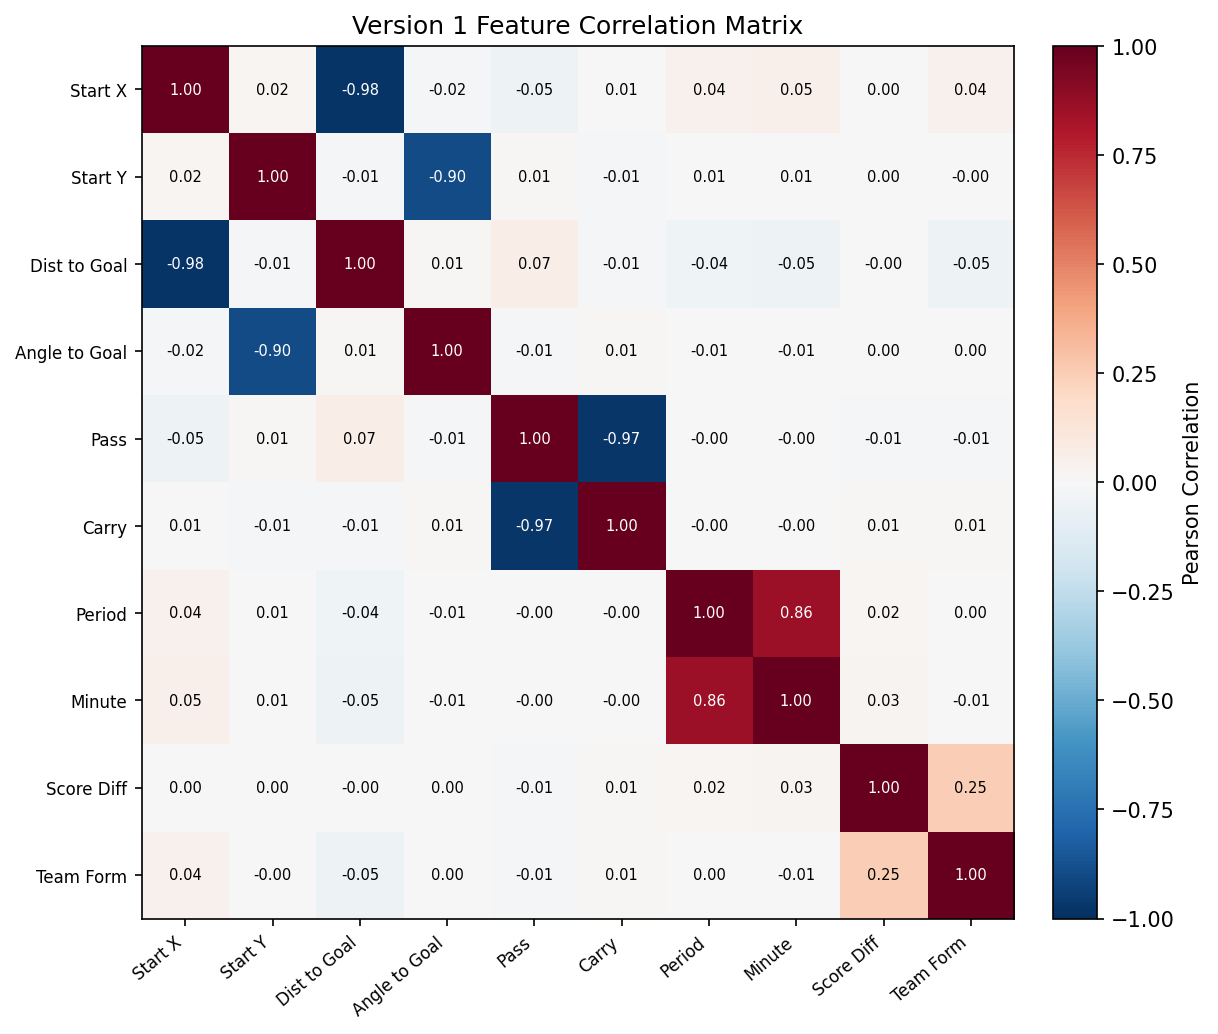
\includegraphics[width=0.72\textwidth]{xT_v1/xt_feature_correlation.png}
    \caption{Pearson correlation matrix for Version 1 input features.}
\end{figure}

The matrix reveals three distinct clusters of correlation. First, the spatial features: \texttt{dist\_to\_goal} and \texttt{start\_x} show a very strong negative correlation ($r = -0.98$), since being further up the pitch means being closer to goal. Likewise, \texttt{angle\_to\_goal} and \texttt{start\_y} are strongly correlated ($r = -0.90$), since centrality on the pitch determines the angle. Both pairs carry overlapping information, but each captures a meaningfully different geometric aspect of position, and both were retained since Random Forest is robust to moderate inter-feature correlation.

Second, the action-type flags: \texttt{type\_Pass} and \texttt{type\_Carry} show a near-perfect negative correlation ($r = -0.97$). This is a direct consequence of one-hot encoding: for any given event, if it is a pass, it cannot be a carry, and vice versa. Shot events (excluded from training features) receive zeros for both, which prevents the correlation from reaching exactly $-1.0$. Despite this redundancy, both flags were retained to preserve an explicit positive signal for each action type.

Third, the time features: \texttt{period} and \texttt{minute} are strongly correlated ($r = 0.86$), as the minute increases monotonically within each period. The remaining context features (\texttt{score\_diff}, \texttt{team\_form}) are nearly orthogonal to all spatial and time features. There is a mild positive correlation between \texttt{score\_diff} and \texttt{team\_form} ($r = 0.25$), reflecting that better-performing teams tend to lead more often, but this is too weak to cause concern.

% ============================================================
\section{Evaluation Methodology}\label{sec:eval}
% ============================================================
% TODO: This section should appear before the model chapters so the reader
% understands how results will be reported before seeing them.
% Aim for ~1 page.

\subsection{Evaluation Metrics}
% TODO: Define and justify each of the four metrics used. For each one, state:
%   (a) its mathematical definition
%   (b) its range and what good/bad looks like
%   (c) why it is appropriate for an xT model specifically

\subsubsection{ROC AUC}

ROC AUC (Area Under the Receiver Operating Characteristic Curve) measures how well the model can separate goal-chain events from non-goal-chain events, regardless of any specific probability threshold. A score of 0.5 means the model performs no better than random, while a score of 1.0 means perfect separation. Because we are ultimately interested in whether high-threat events receive higher scores than low-threat events, this is a natural metric for an xT model.

For Versions 2 and 3, the training labels are soft floating-point values produced by temporal discounting, not the binary 0/1 labels that ROC AUC expects. We therefore binarise the labels before computing the metric: any event with a label greater than zero (i.e., any event that appeared in a goal-scoring chain) is treated as a positive. This is a principled choice: it preserves the intended semantics of the label while making the metric computable.

\subsubsection{Brier Score}

The Brier Score is the mean squared error between the model's predicted probability $\hat{p}$ and the true label $y$:

\[
\text{BS} = \frac{1}{N} \sum_{i=1}^{N} (\hat{p}_i - y_i)^2
\]

It ranges from 0 (perfect predictions) to 1 (worst possible). Unlike ROC AUC, which only cares about ranking, the Brier Score also penalises poor calibration. For example, a model that assigns a probability of 0.9 to an event that does not lead to a goal is penalised more than one that assigns 0.6 to the same event. This makes it a useful complement to ROC AUC: a model can have a high AUC but a poor Brier Score if its predicted probabilities are systematically over-confident.

\subsubsection{Log Loss (Binary Cross-Entropy)}

Log Loss, also known as binary cross-entropy, penalises confident wrong predictions much more heavily than the Brier Score does. The formula is:

\[
\text{Log Loss} = -\frac{1}{N} \sum_{i=1}^{N} \left[ y_i \log(\hat{p}_i) + (1 - y_i) \log(1 - \hat{p}_i) \right]
\]

A model that assigns $\hat{p} = 0.99$ to an event that does not score will receive a very large penalty, whereas the same error with $\hat{p} = 0.6$ receives a much smaller one. This makes log loss a sensitive measure of overconfidence.

We compute this manually rather than using \texttt{sklearn}'s built-in \texttt{log\_loss}, because scikit-learn rejects continuous floating-point labels and expects binary values. Our implementation handles the soft labels used in Versions 2 and 3 directly, treating them as the interpolated positive probability they were intended to represent. Predicted probabilities are clipped to $[10^{-7}, 1 - 10^{-7}]$ before taking the logarithm to prevent numerical instability.

\subsubsection{Spearman Rank Correlation ($\rho$)}

Spearman's $\rho$ measures the rank correlation between predicted probabilities and true labels. Rather than comparing the raw values directly, it first converts both sequences into rank orderings and then computes the Pearson correlation of those ranks. It ranges from $-1$ (perfect inverse ranking) through $0$ (no relationship) to $+1$ (perfect ranking).

For an xT model, ranking quality matters: we want the model to correctly order events by threat level: a carry into the box should score higher than a pass in the defensive third. Spearman $\rho$ captures this directly. However, because the label distribution is extremely imbalanced (only 0.32\% of events belong to a goal chain), $\rho$ values tend to be low in absolute terms even for a well-performing model. The vast majority of events have a label of zero, so even a model that perfectly separates the positive class will have its rank correlation diluted across 99.68\% of uninformative pairs. For this reason, \textbf{ROC AUC is the primary evaluation metric} used to compare model quality across versions; it directly measures whether the model ranks goal-chain events above background events, ignoring the within-group ordering that contributes noise. Spearman $\rho$ is used as the training signal for Versions 2 and 3 (the \texttt{ReduceLROnPlateau} scheduler monitors it), but ROC AUC is the headline number when interpreting results.

\subsection{Cross-Version Comparison Design}

To make the results across all three versions directly comparable, we took several deliberate design decisions.

All three versions use the same 70/15/15 train/validation/test split, performed at the match level with a fixed random seed of 42. Splitting at the match level is important to prevent data leakage: if events from the same match could appear in both the training and test sets, the model might implicitly memorise match-specific patterns rather than learning general football behaviour. Using a fixed seed means the split is reproducible and the same for every version.

For Versions 2 and 3, which both use the 360 freeze-frame dataset, we go one step further: Version 3 saves its exact test match IDs to a \texttt{test\_match\_ids.json} file at training time, and Version 2's evaluation script loads those same IDs to restrict its test set to the same 49 matches. This means any difference in the Version 2 and Version 3 test metrics reflects a genuine difference in model quality, not a difference in which events were evaluated.

Version 1 uses a different test set: all events from 15\% of the full 3,464-match dataset, roughly 521 matches. This is intentional: Version 1 predates the 360 data requirement, so it is evaluated on the broader event population it was built for. The step from Version 1 to Version 2 therefore combines both an architecture improvement and a data upgrade to 360 matches, while the step from Version 2 to Version 3 is a pure architecture comparison on identical data.

Finally, all four metrics for all three versions are computed by the same shared \texttt{evaluate.py} module, so there is no risk of inconsistency in how metrics are calculated between versions.

% ============================================================
\section{Version 1: Random Forest}\label{sec:v1}
% ============================================================

\subsection{Data Preparation}

In order to do this, we have to process the files, as they are currently stored in JSON format, and in order to integrate with Python's NumPy and Pandas libraries, we will need to transform the data into a CSV file for Python to read. This CSV file will contain all of the features we have decided on, as well as the values they hold for each unique event.

We will also need to chain these events together, as mentioned in Section~\ref{sec:dataset}, so we can determine our output feature : whether the chain resulted in a loss of possession, or a goal. This involves checking each play in each game by the timestamp, and setting the output to 1 when it parses a goal in the JSON file, and setting the output to 0 in other scenarios when the attacking team loses possession.

\subsection{Model Architecture and Design Choices}

After the data was processed, the next step was to train a model to predict the likelihood of scoring. For this initial iteration, a Random Forest model was selected. This algorithm generates multiple decision trees and aggregates their outputs to produce a single prediction. Prior to training, the data was partitioned into training and validation sets, and appropriate metrics were established to effectively evaluate the model's performance.

The dataset is split at the match level using a 70/15/15 train/validation/test partition with a fixed seed (42), matching the split used by all three model versions. Entire matches belong to exactly one partition, which prevents data leakage that would arise if events from the same match appeared in both the training and test sets. Version 1 does not use a validation loop (Random Forests have no early stopping), so the validation matches are withheld from training but not used during the training process itself.

To assess model performance, ROC AUC and Brier Score were utilised. ROC plots the True Positive Rate against the False Positive Rate, where the ROC AUC score is given by the area under the curve. A score of 1 indicates a perfect model, whereas a score of 0.5 indicates random predictions. The Brier Score evaluates the accuracy of predictions for binary outcomes by taking the mean squared difference between predicted probabilities and actual outcomes, ranging from the best possible score of 0 to the worst possible score of 1.

Using both of these evaluation metrics, we should be able to get a very solid inference of how well our model is working, but to fully ensure, I will also make sure to generate a heatmap when we have finished training to predict the likelihood of scoring from each position on the pitch, and line it up with what logically makes sense.

\subsection{Results}

Version 1 achieved a test ROC AUC of \textbf{0.6828}, Brier Score of \textbf{0.0159}, Log Loss of \textbf{0.0795}, and Spearman $\rho$ of \textbf{0.0810}. The ROC AUC of 0.68 is a moderate improvement over random (0.5), confirming the model can distinguish goal-chain events from background possession. The low Spearman $\rho$ reflects the difficulty of ranking fine-grained possession events with tabular features alone; see Section~\ref{sec:comparison} for a full cross-version comparison.

\begin{figure}[h]
    \centering
    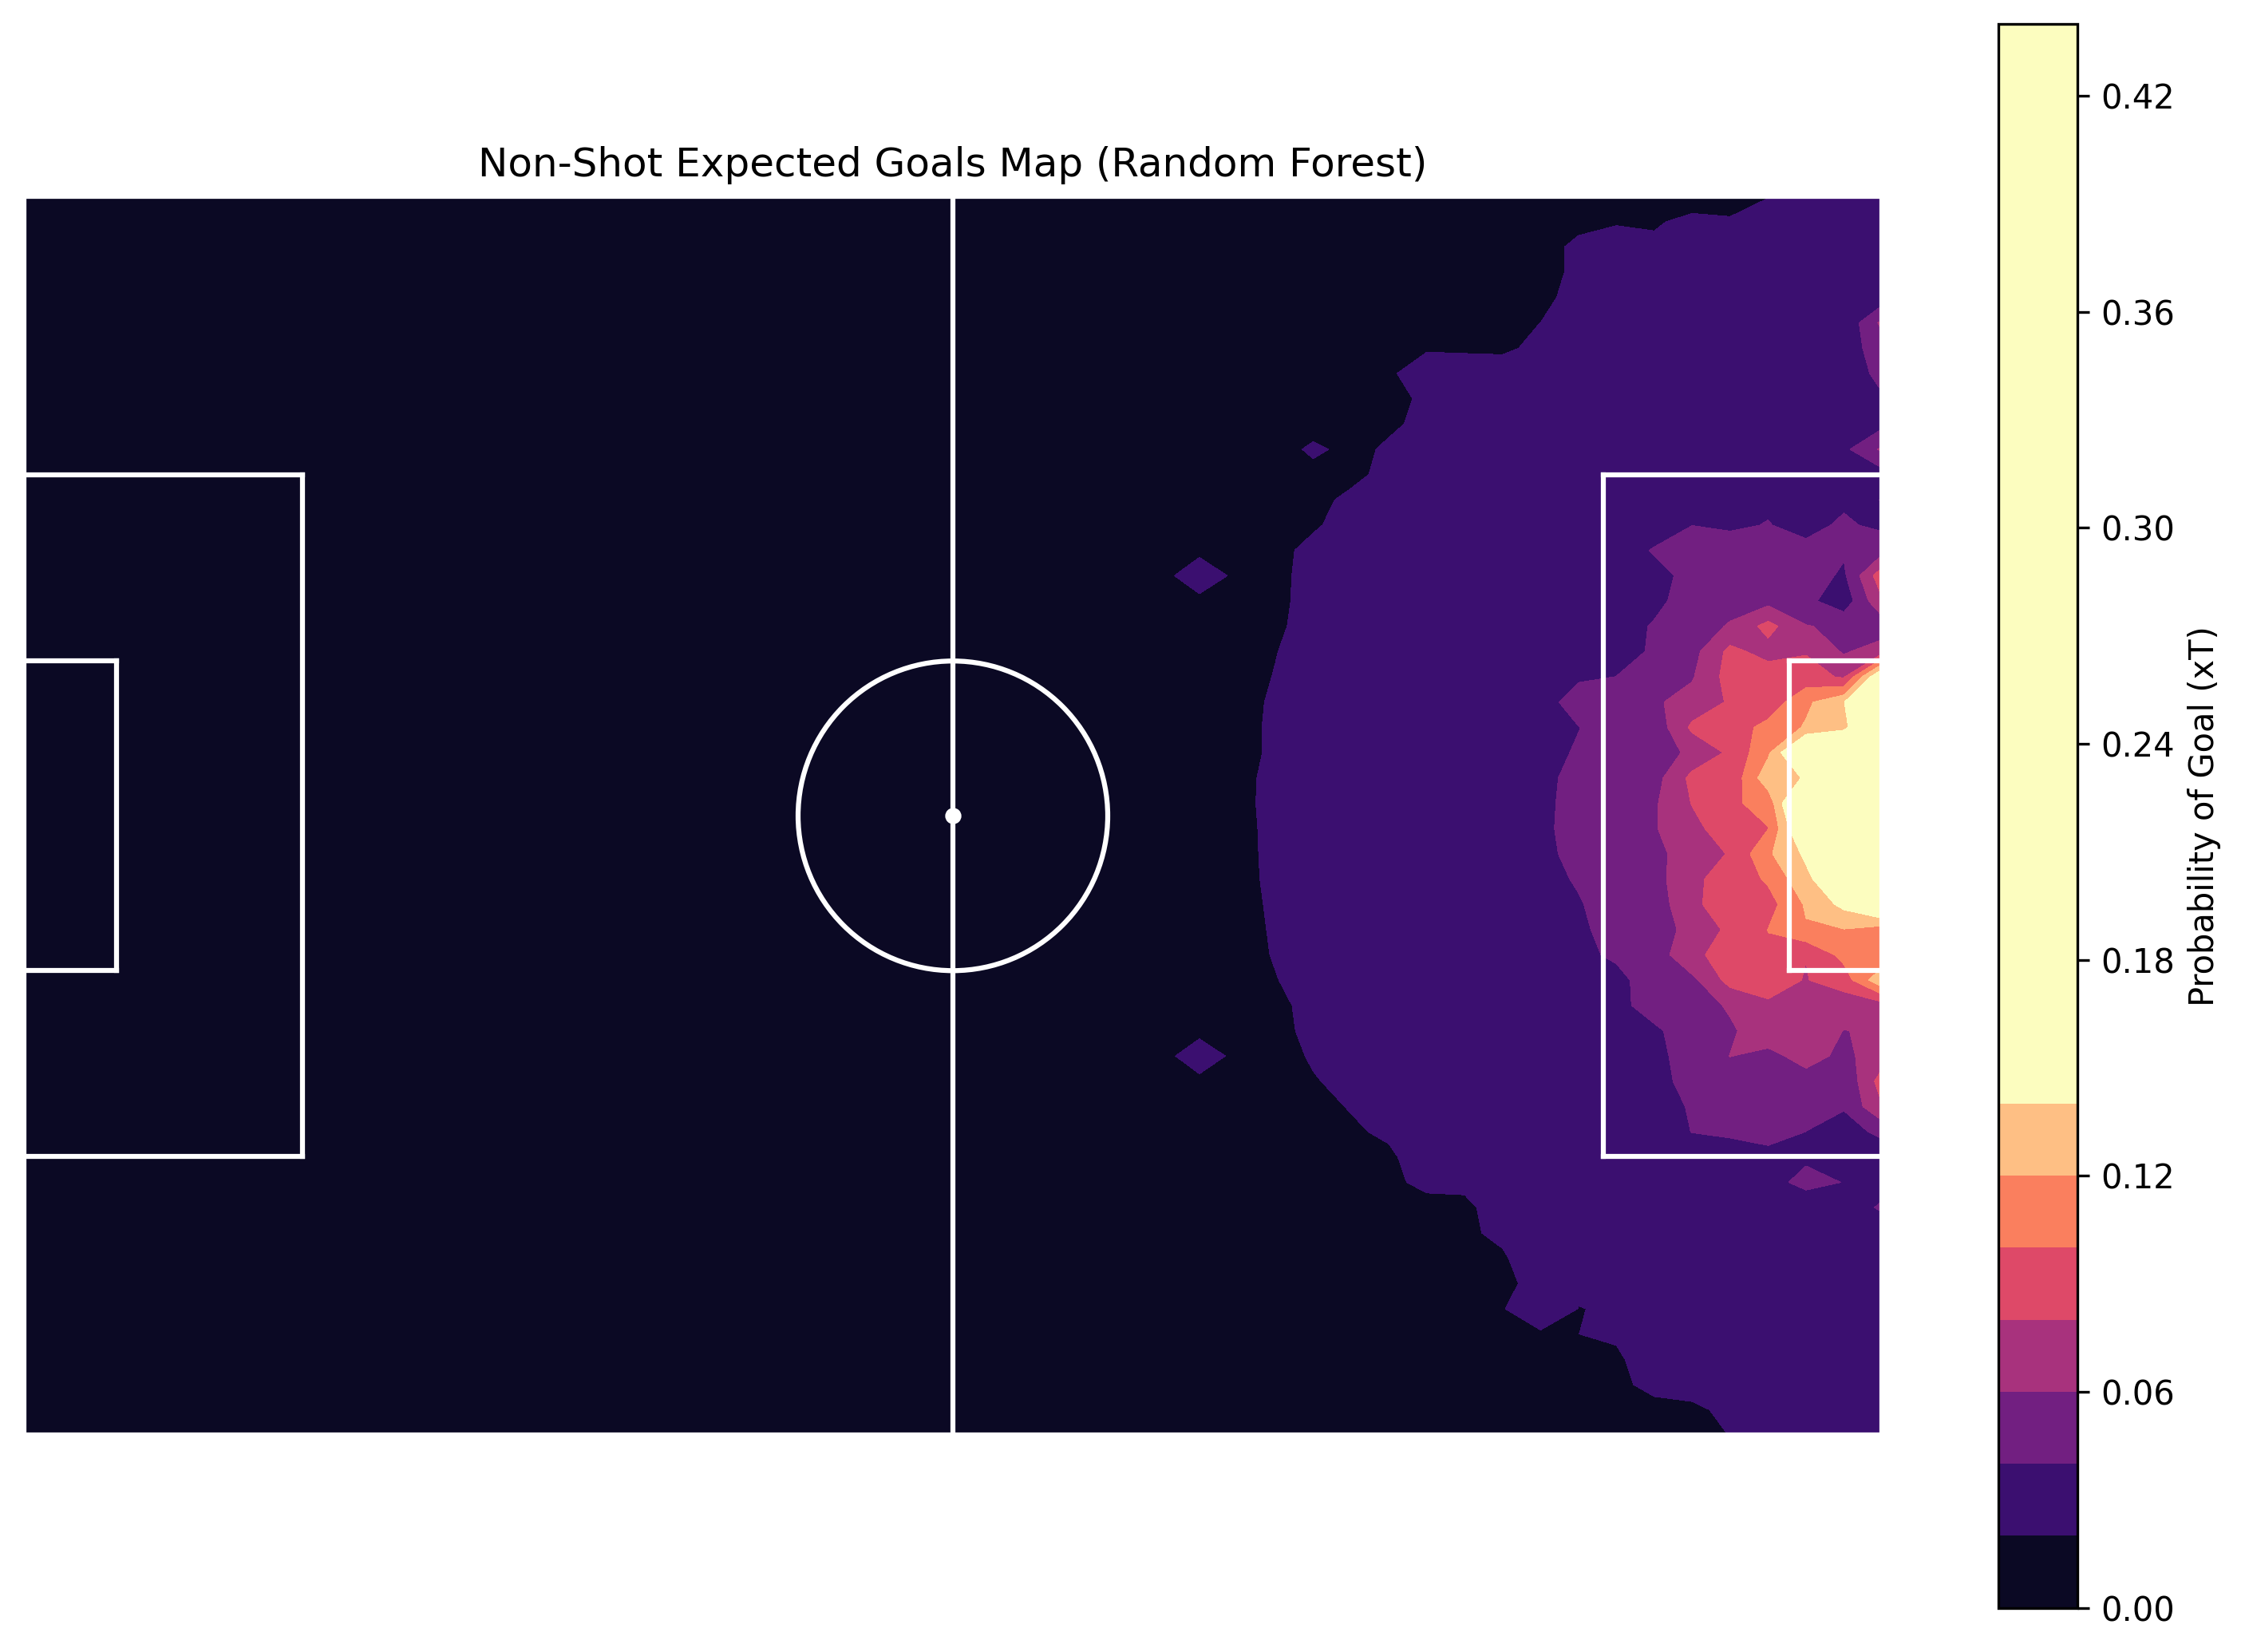
\includegraphics[width=0.8\textwidth]{xT_v1/xt_heatmap.png}
    \caption{Non-Shot xT Heatmap: Version 1 (Random Forest), assuming a Pass action type at a neutral game state (period 2, minute 45, score level, average team form).}
\end{figure}

The heatmap confirms that the model has learned a broadly sensible spatial representation: threat is concentrated in and around the attacking penalty area, peaks just in front of the 6-yard box, and drops off sharply as the ball moves deeper or wider. The defensive half is effectively zero throughout. This is consistent with the feature importance analysis showing that \texttt{dist\_to\_goal} accounts for nearly 40\% of the model's predictive power.

However, the Random Forest's decision-tree structure is also visible: rather than a perfectly smooth radial gradient, the threat surface has jagged, stepped edges and a handful of small elevated regions around the midfield area (visible as isolated blobs). These are artefacts of the ensemble of axis-aligned decision boundaries that a Random Forest produces, and confirm that the model has not learned a true continuous spatial representation. This motivates the move to a CNN in Version 2, which can learn genuinely smooth spatial features directly from data.

\subsection{Feature Importance}

It is also very important that we check how much each feature in this Random Forest Model actually contributes to our final data, as it could be that all of the information has been gained by just one feature, which can tell us as well if we are including features that aren't at all necessary. In the following, we can see the results.

\begin{figure}[h]
    \centering
    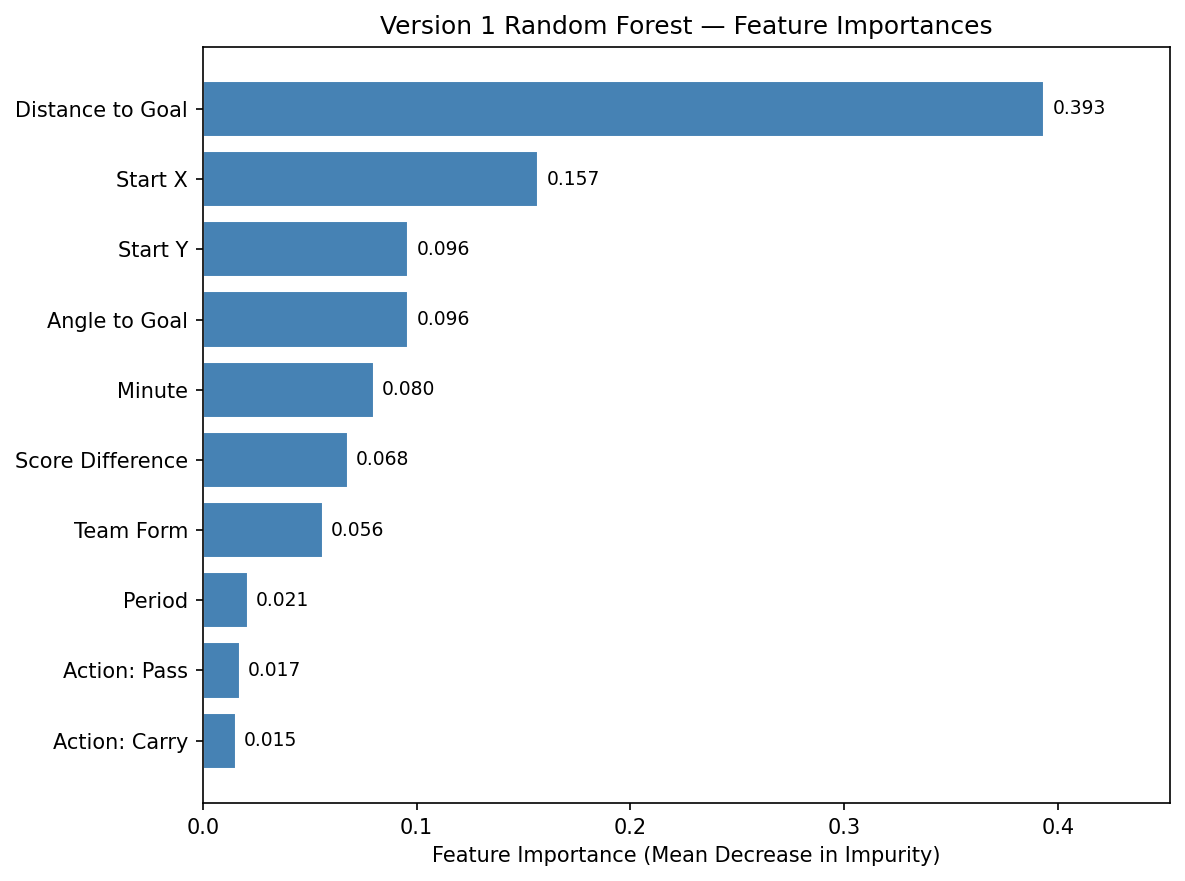
\includegraphics[width=0.85\textwidth]{xT_v1/xt_feature_importance.png}
    \caption{Feature importance scores for the Version 1 Random Forest model (mean decrease in impurity).}
\end{figure}

The feature importance results reveal a clear hierarchy. \texttt{dist\_to\_goal} is overwhelmingly dominant at 0.393, accounting for nearly 40\% of the total impurity reduction on its own. \texttt{start\_x} is a distant second at 0.157, followed by \texttt{start\_y} and \texttt{angle\_to\_goal} which are essentially tied at 0.096 each.

Notably, the three main context features contribute meaningfully rather than marginally: \texttt{minute} scores 0.080, \texttt{score\_diff} 0.068, and \texttt{team\_form} 0.056. Together these three account for roughly 20\% of total importance, comparable to the combined contribution of \texttt{start\_x}. This confirms that game-state context is a genuine signal for xT prediction: later in a match and under greater pressure to score, attacking sequences are more threatening for a given ball position. \texttt{period} is the one context feature that contributes minimally (0.021), likely because \texttt{minute} already encodes the same information more continuously.

The action type flags (\texttt{type\_Pass} at 0.017, \texttt{type\_Carry} at 0.015) contribute the least. Since the dataset contains only passes, carries, and shots (and shots are excluded from training features), the distinction between a pass and a carry adds relatively little once position is already known. Overall, the model has learned a distance-to-goal heuristic enriched by a meaningful contextual adjustment, though the richer information that would most help (player positions, passing lanes, defensive pressure) remains absent from this version.

\subsection{Limitations and Motivation for Version 2}

The results highlight several fundamental limitations with the Version 1 model. Distance to goal alone accounts for nearly 40\% of the model's predictive power, and the top four spatial features (\texttt{dist\_to\_goal}, \texttt{start\_x}, \texttt{start\_y}, \texttt{angle\_to\_goal}) together account for roughly 74\%. The context features (\texttt{minute}, \texttt{score\_diff}, \texttt{team\_form}) add a genuine but secondary contribution of around 20\%, while \texttt{period} and the action-type flags contribute very little. The model also ignores the other players' positional data completely. Incorporating it would require a richer representation than a flat scalar feature vector: a Random Forest cannot learn the complex spatial relationships between each of the players and the ball from a list of numbers alone.

% ============================================================
\section{Version 2: CNN + MLP}\label{sec:v2}
% ============================================================

\subsection{Motivation}

Given the limitations of the Random Forest approach, the logical next step is to move to a neural network that can represent player positions spatially rather than as a flat feature vector. Instead of encoding ``there are 3 defenders within 10 metres'' as a scalar, we can encode the full pitch as an image with each player as a Gaussian blob, and use a Convolutional Neural Network (CNN) to learn the spatial patterns directly.

This also motivates a switch to the StatsBomb 360 dataset, which provides freeze-frame snapshots at the moment of every tracked event, giving us the actual positions of all visible players on the pitch rather than just the ball.

The evaluation framework also evolves for Version 2. Because we now use temporally discounted soft labels ($\gamma^k$) rather than binary chain outcomes, we use \textbf{Spearman rank correlation ($\rho$)} as the training signal ; it monitors whether the model correctly orders events by their discounted threat value. ROC AUC remains the primary evaluation metric reported for model comparison, with the soft labels binarised (label $> 0$ = goal chain) before computing it.

\subsection{Architecture}

The Version 2 model is a dual-branch network:

\begin{itemize}
    \item \textbf{CNN Branch}: Takes the $(6 \times 40 \times 60)$ spatial pitch tensor and processes it through three convolutional blocks (Conv2d $\to$ BatchNorm $\to$ ReLU $\to$ MaxPool), halving spatial dimensions at each stage: $(6,40,60) \to (32,20,30) \to (64,10,15) \to (128,5,7)$. The flattened output is passed through a linear head to produce a 256-dimensional feature vector.
    \item \textbf{MLP Branch}: Takes the 22-dimensional scalar feature vector through two fully-connected layers to produce a 32-dimensional feature vector.
\end{itemize}

The outputs of both branches are concatenated to form a 288-dimensional combined representation, which is passed through a final two-layer classifier to produce a single logit (pre-sigmoid score). The model has \textbf{1,282,369 trainable parameters}.

\begin{figure}[h]
\centering
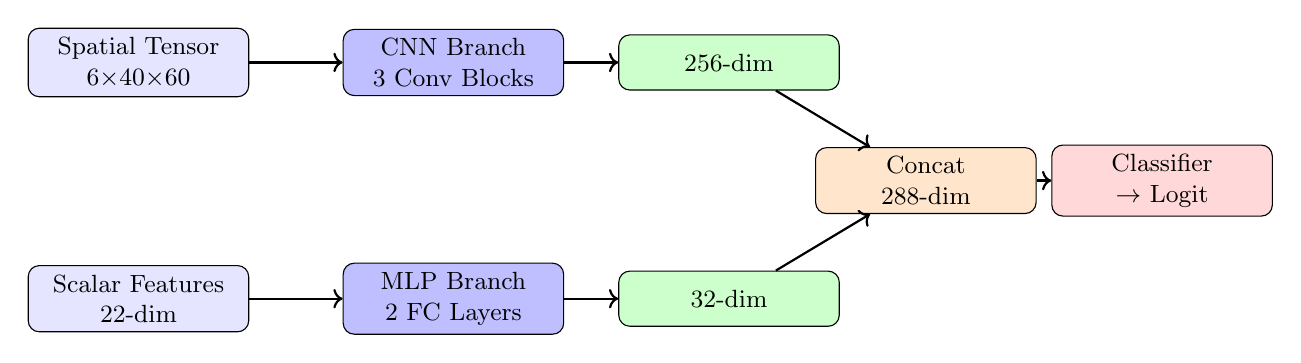
\begin{tikzpicture}[
    box/.style={draw, rounded corners, minimum width=2.8cm, minimum height=0.7cm, align=center, font=\small},
    arr/.style={->, thick}
]
\node[box, fill=blue!10]  (spatial) at (0, 3)    {Spatial Tensor\\$6{\times}40{\times}60$};
\node[box, fill=blue!10]  (scalar)  at (0, 0)    {Scalar Features\\$22$-dim};
\node[box, fill=blue!25]  (cnn)     at (4, 3)    {CNN Branch\\3 Conv Blocks};
\node[box, fill=blue!25]  (mlp)     at (4, 0)    {MLP Branch\\2 FC Layers};
\node[box, fill=green!20] (cnnout)  at (7.5, 3)  {256-dim};
\node[box, fill=green!20] (mlpout)  at (7.5, 0)  {32-dim};
\node[box, fill=orange!20](concat)  at (10, 1.5) {Concat\\288-dim};
\node[box, fill=red!15]   (cls)     at (13, 1.5) {Classifier\\$\to$ Logit};

\draw[arr] (spatial) -- (cnn);
\draw[arr] (scalar)  -- (mlp);
\draw[arr] (cnn)     -- (cnnout);
\draw[arr] (mlp)     -- (mlpout);
\draw[arr] (cnnout)  -- (concat);
\draw[arr] (mlpout)  -- (concat);
\draw[arr] (concat)  -- (cls);
\end{tikzpicture}
\caption{Version 2 dual-branch architecture. The CNN branch processes the spatial pitch tensor; the MLP branch processes scalar context features. Their outputs are concatenated and passed to a final classifier.}
\label{fig:v2arch}
\end{figure}

\subsection{Training}

Training uses \texttt{BCEWithLogitsLoss} with a capped positive class weight to handle severe class imbalance (goal rate: 0.32\%). The positive weight is capped at 10.0 to prevent over-amplification of goal-chain gradients. The optimiser is Adam with a learning rate of $10^{-3}$ and weight decay of $10^{-4}$, with a \texttt{ReduceLROnPlateau} scheduler monitoring validation Spearman $\rho$. Training ran for 50 epochs on an NVIDIA RTX 6000 Ada GPU, with the best model checkpoint saved at each improvement.

The dataset contains \textbf{1,036,140 events} from 323 matches (258 training, 65 validation), split at the match level to prevent data leakage.

\subsection{Results}

Version 2 achieved a test ROC AUC of \textbf{0.8416}, Brier Score of \textbf{0.0067}, Log Loss of \textbf{0.0413}, and Spearman $\rho$ of \textbf{0.0816}. The ROC AUC of 0.84 is a substantial improvement over Version 1 (0.68), confirming that the CNN architecture combined with full player positional context is far better at separating goal-chain events from background possession. The best validation Spearman $\rho$ was 0.0862. Although modest in absolute modest in absolute terms due to the extreme class imbalance, but positive and consistent, indicating the model learns a meaningful threat ordering. The low Brier Score reflects that the model correctly assigns very low probabilities to the vast majority of non-threatening events.

\begin{figure}[h]
    \centering
    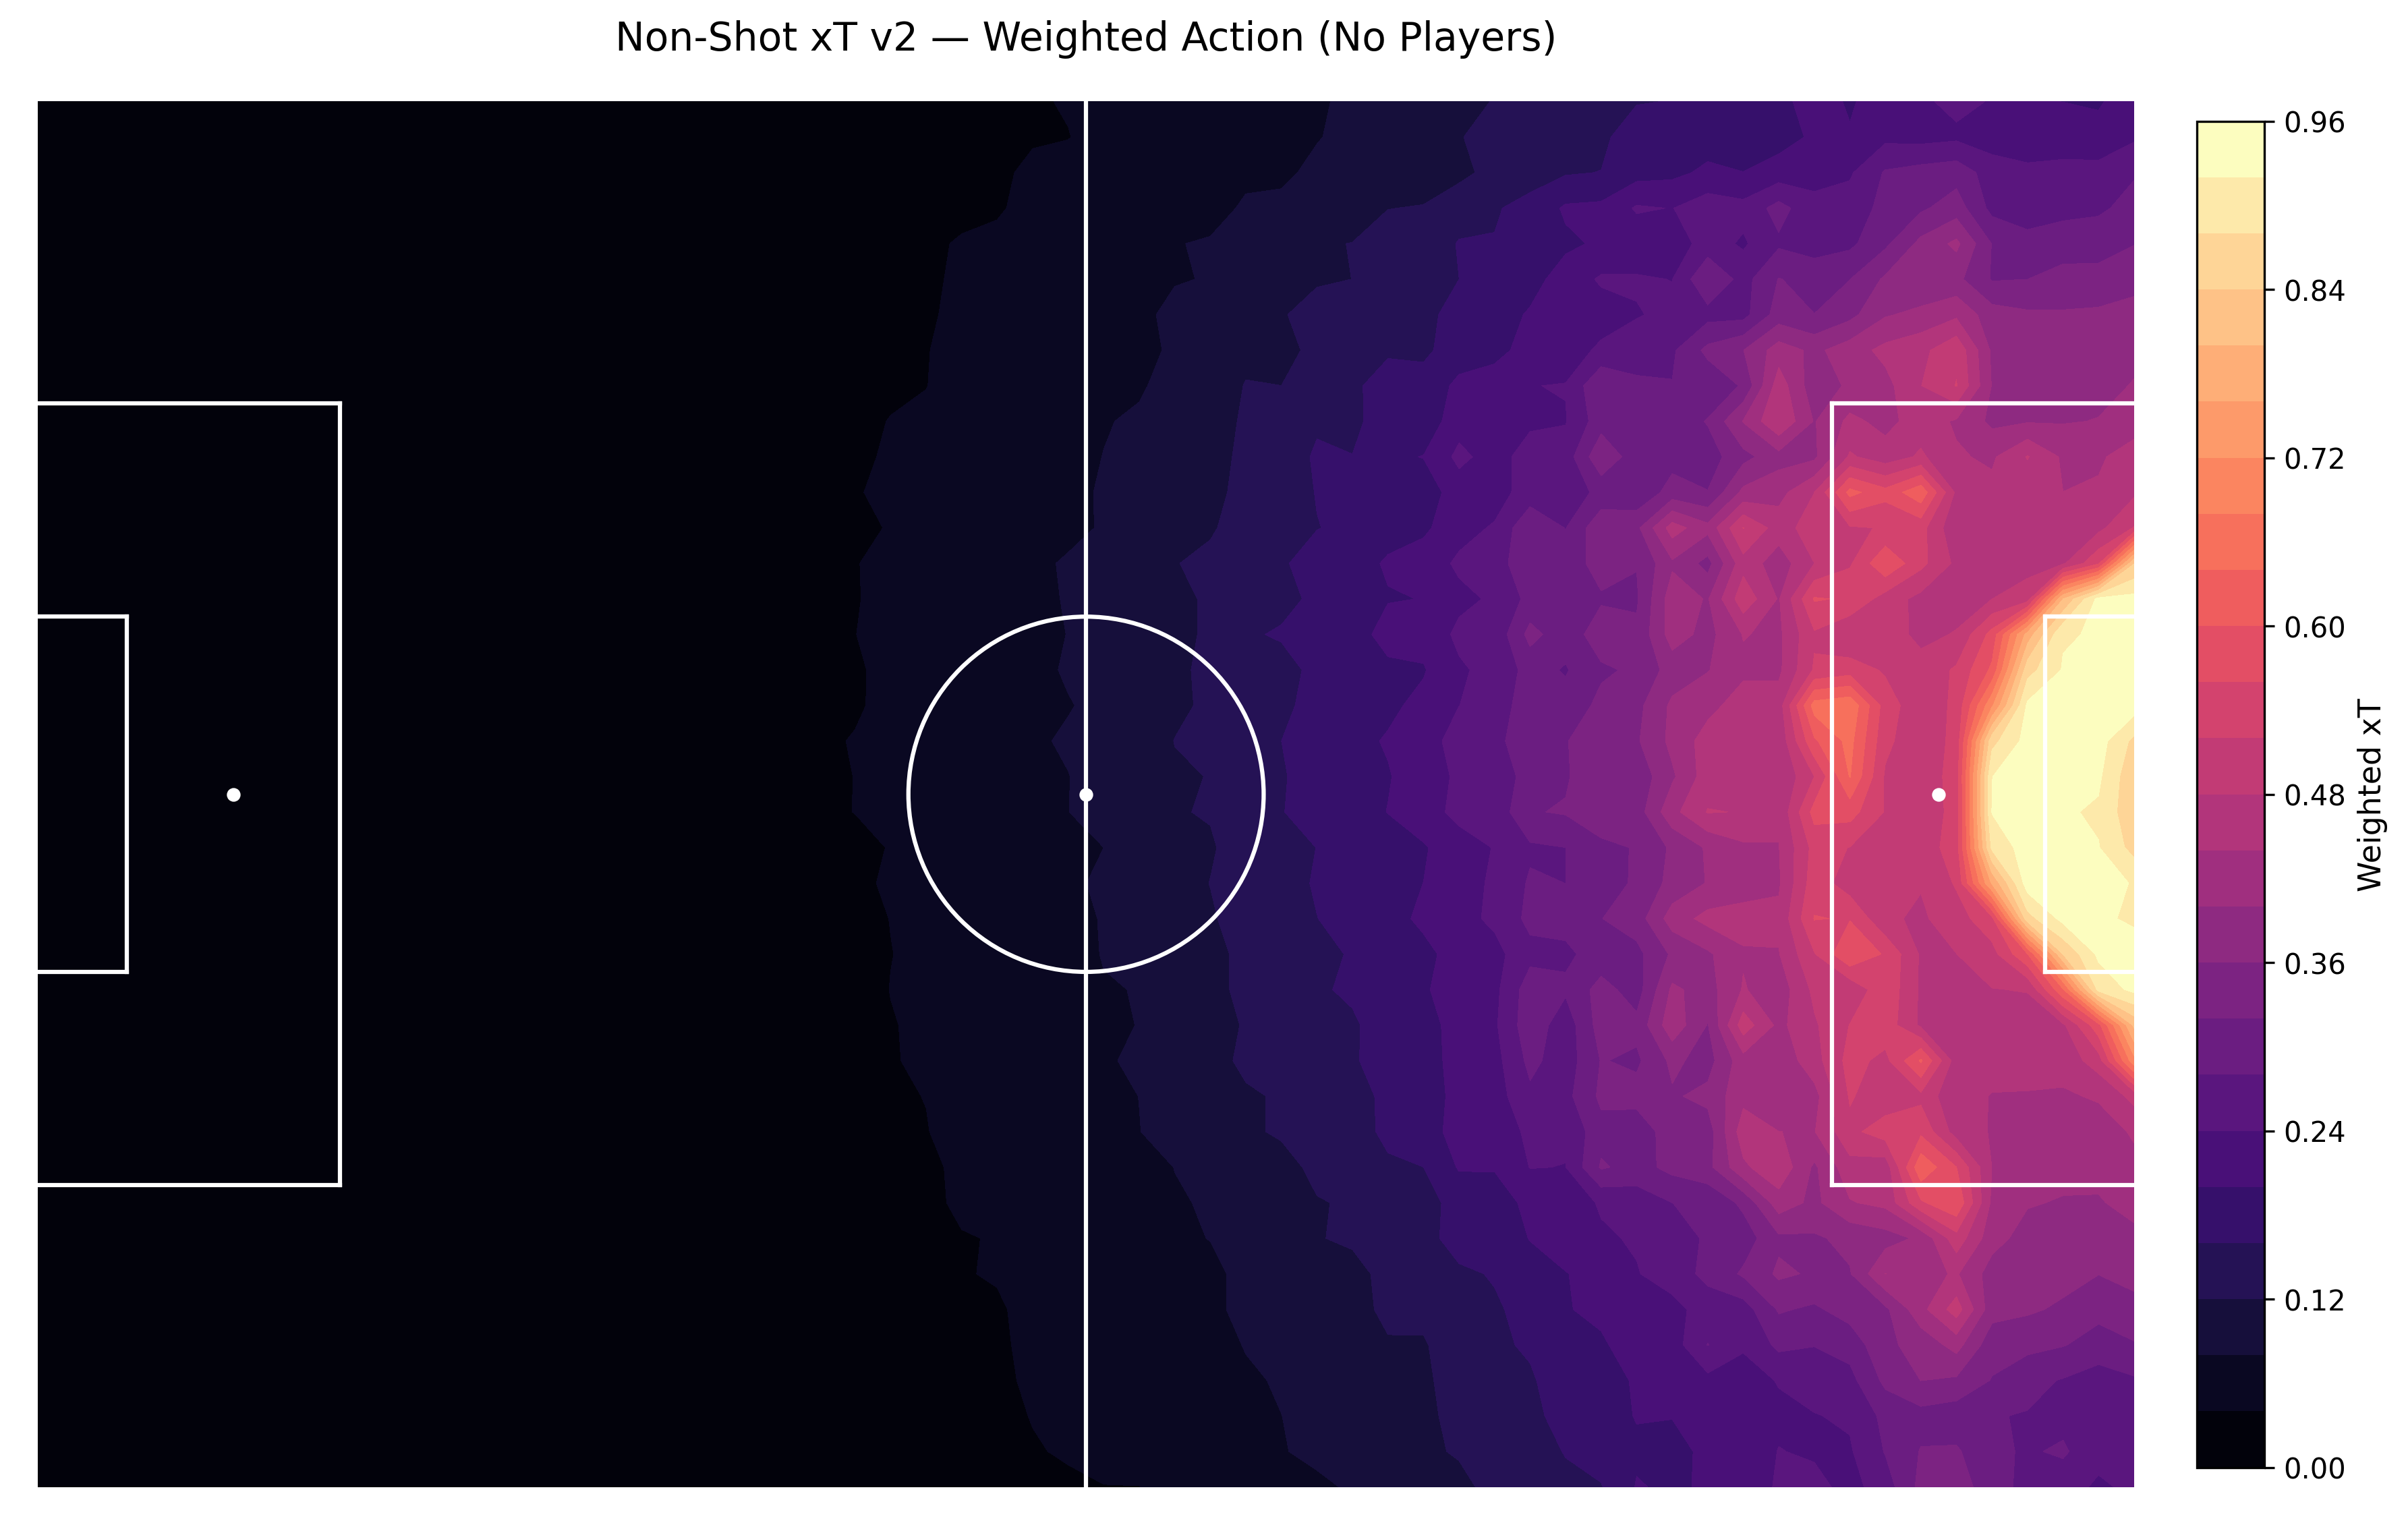
\includegraphics[width=0.8\textwidth]{xT_v2/xt_heatmap_weighted_v2.png}
    \caption{Non-Shot xT Heatmap: Version 2 CNN, weighted action combination (no players, baseline). For each grid cell the model is run under all four action types (Shot, Pass, Carry, Dribble) and the results are combined using position-inferred action weights, identical to the Version 3 and frontend methodology.}
\end{figure}

The Version 2 baseline heatmap (no players present) is strikingly smoother than Version 1. The CNN has learned a continuous, radially symmetric threat surface with threat peaking in the 6-yard box and fading uniformly with distance. There are no decision-tree artefacts or isolated blobs. The colourbar reaches values notably higher than Version 1's peak, reflecting the weighted combination of action types: close to goal, Shot receives a large weight, pulling the combined xT upward beyond what any single action type would produce alone.

\begin{figure}[h]
    \centering
    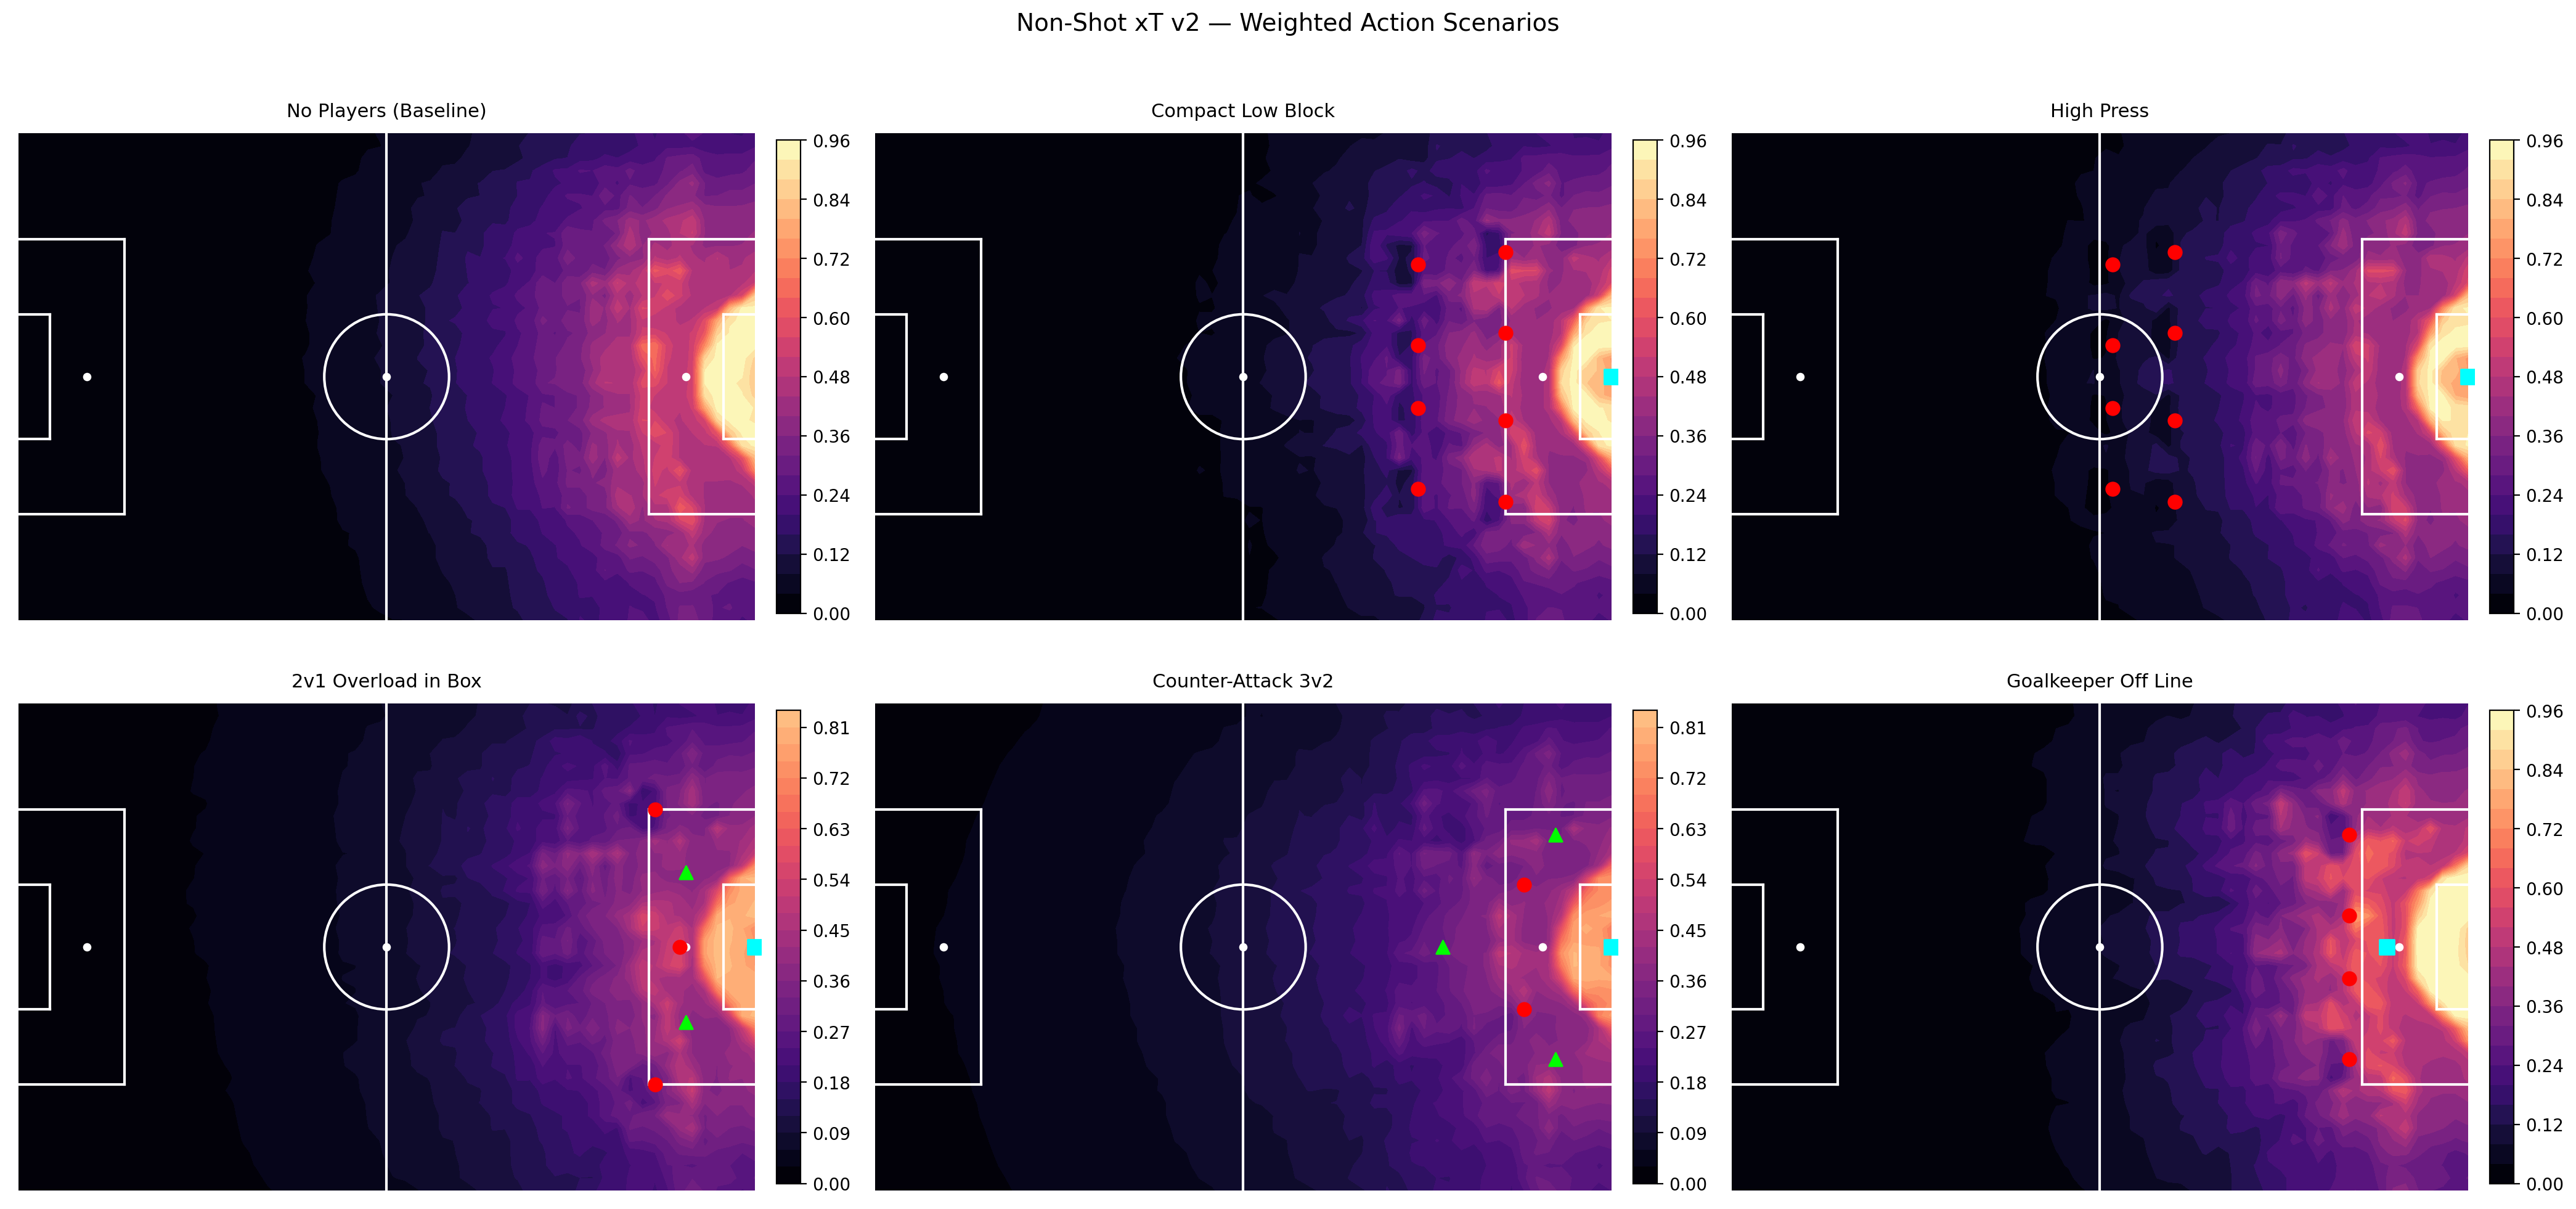
\includegraphics[width=0.8\textwidth]{xT_v2/xt_scenarios_weighted_v2.png}
    \caption{Scenario comparison: Version 2 CNN, weighted xT. Six defensive configurations showing how player positions modulate the combined threat surface.}
\end{figure}

The six scenario panels are the most revealing diagnostic for Version 2's capabilities and limitations.

\textbf{No Players (Baseline).} A smooth, radially symmetric threat surface peaks in the 6-yard box and fades uniformly outward. This is the CNN's learned positional prior: with no player context, threat tracks distance and angle to goal.

\textbf{Compact Low Block.} Eight defenders occupy a tight block at $x = 88$ and $x = 102$, forming two defensive lines directly in front of goal. The threat surface is almost indistinguishable from the no-player baseline. The defenders do lower the Carry weight (high close-defender count) and Shot weight (blocked shooting lane), but because the CNN encodes them as overlapping Gaussian blobs, it cannot distinguish a structured defensive wall from a randomly scattered group of eight players at similar positions. The central channel is not selectively suppressed; the overall threat field remains radially symmetric.

\textbf{High Press.} All eight outfield defenders are positioned at $x = 62$--$72$, well away from the attacking third. The threat surface near goal is identical to the baseline, correctly reflecting that no defenders are present to block shots or carries at close range. However, the panel provides no information about the exposed space immediately behind the high line: because Version 2 encodes players by spatial density rather than individual identity, the model cannot infer that high-positioned defenders imply vulnerability behind them.

\textbf{2v1 Overload in Box.} Two attacking teammates (green triangles at $(108, 28)$ and $(108, 52)$) flank a single defender. Their presence raises the Pass action weight for cells near the penalty area, slightly amplifying threat in that zone relative to the baseline. The single central defender at $(107, 40)$ produces a small local Gaussian in the opponent channel, but it merges into the background density and does not create a visible suppression corridor between ball and goal.

\textbf{Counter-Attack 3v2.} Three attacking teammates spread across different $y$-positions elevate the Pass weight broadly, producing a slightly wider bright zone across the front of the penalty area compared to the baseline. The two covering defenders at $(105, 30)$ and $(105, 50)$ register as a diffuse blob in the opponent channel but do not meaningfully suppress the hot spot.

\textbf{Goalkeeper Off Line.} The keeper is placed at $x = 106$ rather than $x = 119$. The threat surface shows only a subtle difference: the Gaussian representing the keeper is in a different position on the keeper channel, and the CNN responds slightly, but the change is not dramatic. The back four at $x = 100$ produces a familiar density wall that dominates the player context.

Across all six panels the dominant story is similarity. The Version 2 scenario grids look almost like six copies of the same heatmap with dots placed differently on top. This is consistent with the structural limitation discussed below: the CNN processes player positions as a continuous density field, which loses the individual-level relational structure needed to discriminate between defensive formations of equal density but different tactical shape.

\subsection{Limitations and Motivation for Version 3}

Despite using 360 freeze-frame data, Version 2 still has a structural limitation: it encodes player positions as static image channels and relies on the CNN to learn the spatial relationships implicitly. The CNN is good at detecting local spatial patterns in images, but it is not naturally designed to reason about the explicit relationships between individual players (for example, that there is a defender directly between the ball and the goal and two attackers making runs behind the defensive line). This kind of relational reasoning is better suited to an attention-based architecture.

Additionally, while the ROC AUC of 0.8416 is strong, there is still room for improvement. The model captures broad positional threat correctly but may not be fully leveraging the player position information available in the 360 data, since encoding players as a blurred density map loses the individual-level relational structure between them.

% ============================================================
\section{Version 3: Transformer}\label{sec:v3}
% ============================================================

\subsection{Motivation}

The key limitation of the CNN approach is that player positions are encoded as spatial density maps: each player becomes a Gaussian blob in the image, and the CNN must learn from the shape of the resulting density field. This makes it difficult for the model to distinguish between, say, ``two defenders in the penalty area'' and ``one defender directly blocking the shot and one standing wide.'' A Transformer with attention can reason about each player as an individual token and model their pairwise relationships explicitly.

Version 3 therefore introduces a \textbf{two-stage architecture}:
\begin{enumerate}
    \item \textbf{Stage 1}: The frozen Version 2 CNN, which provides a baseline position-based threat estimate.
    \item \textbf{Stage 2}: A small Transformer that reads the 360 freeze-frame player positions as a sequence of tokens, uses self-attention to model relationships between players, and then uses cross-attention to let the ball position query that player context, producing a residual adjustment to the Stage 1 logit.
\end{enumerate}

Only Stage 2 is trained in Version 3; Stage 1 weights are frozen. This means the model starts from a strong position-based baseline and learns only to adjust it based on player context, which reduces the risk of overfitting and keeps the training tractable.

\subsection{Architecture}

\textbf{Player token encoding:} Each player in the freeze frame is encoded as a 5-dimensional vector: $[\texttt{x\_norm},\ \texttt{y\_norm},\ \texttt{is\_teammate},\ \texttt{is\_keeper},\ \texttt{is\_actor}]$. Up to 22 players are included per event; if fewer are present, padding tokens are added with a padding mask so the Transformer ignores them.

\textbf{Stage 2 Transformer (trainable):}
\begin{itemize}
    \item \textbf{Player embedding}: Linear projection from 5-dim player tokens to a $D_{model} = 64$ embedding space.
    \item \textbf{Ball embedding}: Linear projection from 4 ball features (position + distance/angle to goal) to the same 64-dim space.
    \item \textbf{Player self-attention}: A 2-layer Transformer encoder ($N_{heads} = 4$, feed-forward dim = 256, dropout = 0.1) allows players to attend to each other.
    \item \textbf{Cross-attention}: The ball position queries the player context using multi-head attention, producing a 64-dim context vector representing ``what the player positions tell us about this ball position.''
    \item \textbf{Fusion MLP}: The 64-dim context vector is concatenated with the Stage 1 logit and passed through a 2-layer MLP ($64 \to 1$) to produce a residual adjustment. The final output layer is initialised with near-zero weights so Stage 2 begins as a small correction on top of Stage 1.
\end{itemize}

The final model output is $\text{logit}_{v3} = \text{logit}_{v2} + \text{adjustment}$.

\begin{figure}[h]
\centering
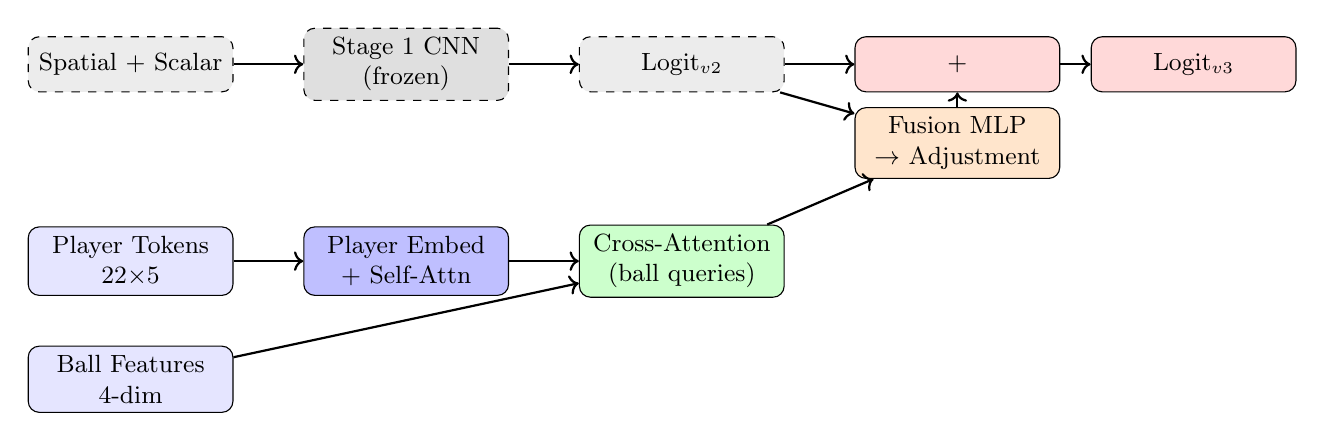
\begin{tikzpicture}[
    box/.style={draw, rounded corners, minimum width=2.6cm, minimum height=0.7cm, align=center, font=\small},
    frozen/.style={draw, rounded corners, minimum width=2.6cm, minimum height=0.7cm, align=center, font=\small, dashed},
    arr/.style={->, thick}
]
% Stage 1 (frozen)
\node[frozen, fill=gray!15]  (sp)     at (0, 4)    {Spatial + Scalar};
\node[frozen, fill=gray!25]  (v2)     at (3.5, 4)  {Stage 1 CNN\\(frozen)};
\node[frozen, fill=gray!15]  (logit1) at (7, 4)    {Logit$_{v2}$};

% Stage 2 (trainable)
\node[box, fill=blue!10]  (ptok)   at (0, 1.5)  {Player Tokens\\$22{\times}5$};
\node[box, fill=blue!25]  (embed)  at (3.5, 1.5){Player Embed\\+ Self-Attn};
\node[box, fill=blue!10]  (ball)   at (0, 0)    {Ball Features\\$4$-dim};
\node[box, fill=green!20] (cross)  at (7, 1.5)  {Cross-Attention\\(ball queries)};
\node[box, fill=orange!20](fusion) at (10.5,3)  {Fusion MLP\\$\to$ Adjustment};

% Output
\node[box, fill=red!15]   (add)    at (10.5, 4) {$+$};
\node[box, fill=red!15]   (out)    at (13.5, 4) {Logit$_{v3}$};

\draw[arr] (sp)     -- (v2);
\draw[arr] (v2)     -- (logit1);
\draw[arr] (logit1) -- (add);
\draw[arr] (ptok)   -- (embed);
\draw[arr] (ball)   -- (cross);
\draw[arr] (embed)  -- (cross);
\draw[arr] (cross)  -- (fusion);
\draw[arr] (logit1) -- (fusion);
\draw[arr] (fusion) -- (add);
\draw[arr] (add)    -- (out);
\end{tikzpicture}
\caption{Version 3 two-stage architecture. The frozen Stage 1 CNN (dashed) produces a baseline logit. Stage 2 encodes player tokens via self-attention, then uses the ball position to query player context via cross-attention; the resulting adjustment is added to the Stage 1 logit.}
\label{fig:v3arch}
\end{figure}

\subsection{Training}

Training procedure mirrors Version 2: \texttt{BCEWithLogitsLoss} with capped positive class weight, Adam optimiser (learning rate $5 \times 10^{-4}$, weight decay $10^{-4}$), \texttt{ReduceLROnPlateau}, and 40 training epochs. Only events with a 360 freeze frame are included in the Version 3 dataset, as player tokens are required for Stage 2. Each epoch logs both the full Version 3 Spearman $\rho$ and the Stage 1 baseline Spearman $\rho$ on the same freeze-frame events, giving a direct measure of how much Stage 2 adds ($\Delta\rho$).

\subsection{Results}

Version 3 achieved a test ROC AUC of \textbf{0.8459}, Brier Score of \textbf{0.0045}, Log Loss of \textbf{0.0302}, and Spearman $\rho$ of \textbf{0.0843}, evaluated on the same 49 freeze-frame test matches (140,697 events) as Version 2.

The Stage 1 (frozen CNN) baseline Spearman $\rho$ on the freeze-frame validation events was 0.0863. Stage 2 training over 40 epochs produced a consistent $\Delta\rho \approx -0.0002$ relative to that baseline, meaning the Transformer cross-attention did not meaningfully improve rank correlation above the CNN alone. The best validation Spearman $\rho$ achieved was 0.0862 (epoch 1). Despite this flat $\rho$, the Brier and Log Loss metrics both improve over Version 2 (0.0067 $\to$ 0.0045 and 0.0413 $\to$ 0.0302), suggesting the Transformer is refining the probability calibration of the CNN's output without changing its ranking order.

% TODO: If time permits, discuss possible reasons: (1) the freeze-frame token encoding
% may not capture enough relational structure for the cross-attention to exploit;
% (2) 40 epochs on 637,926 events may not be sufficient for Stage 2 to converge;
% (3) Spearman rho as a metric may be less sensitive to the fine-grained adjustments
% that player-context conditioning introduces.

\begin{figure}[h]
    \centering
    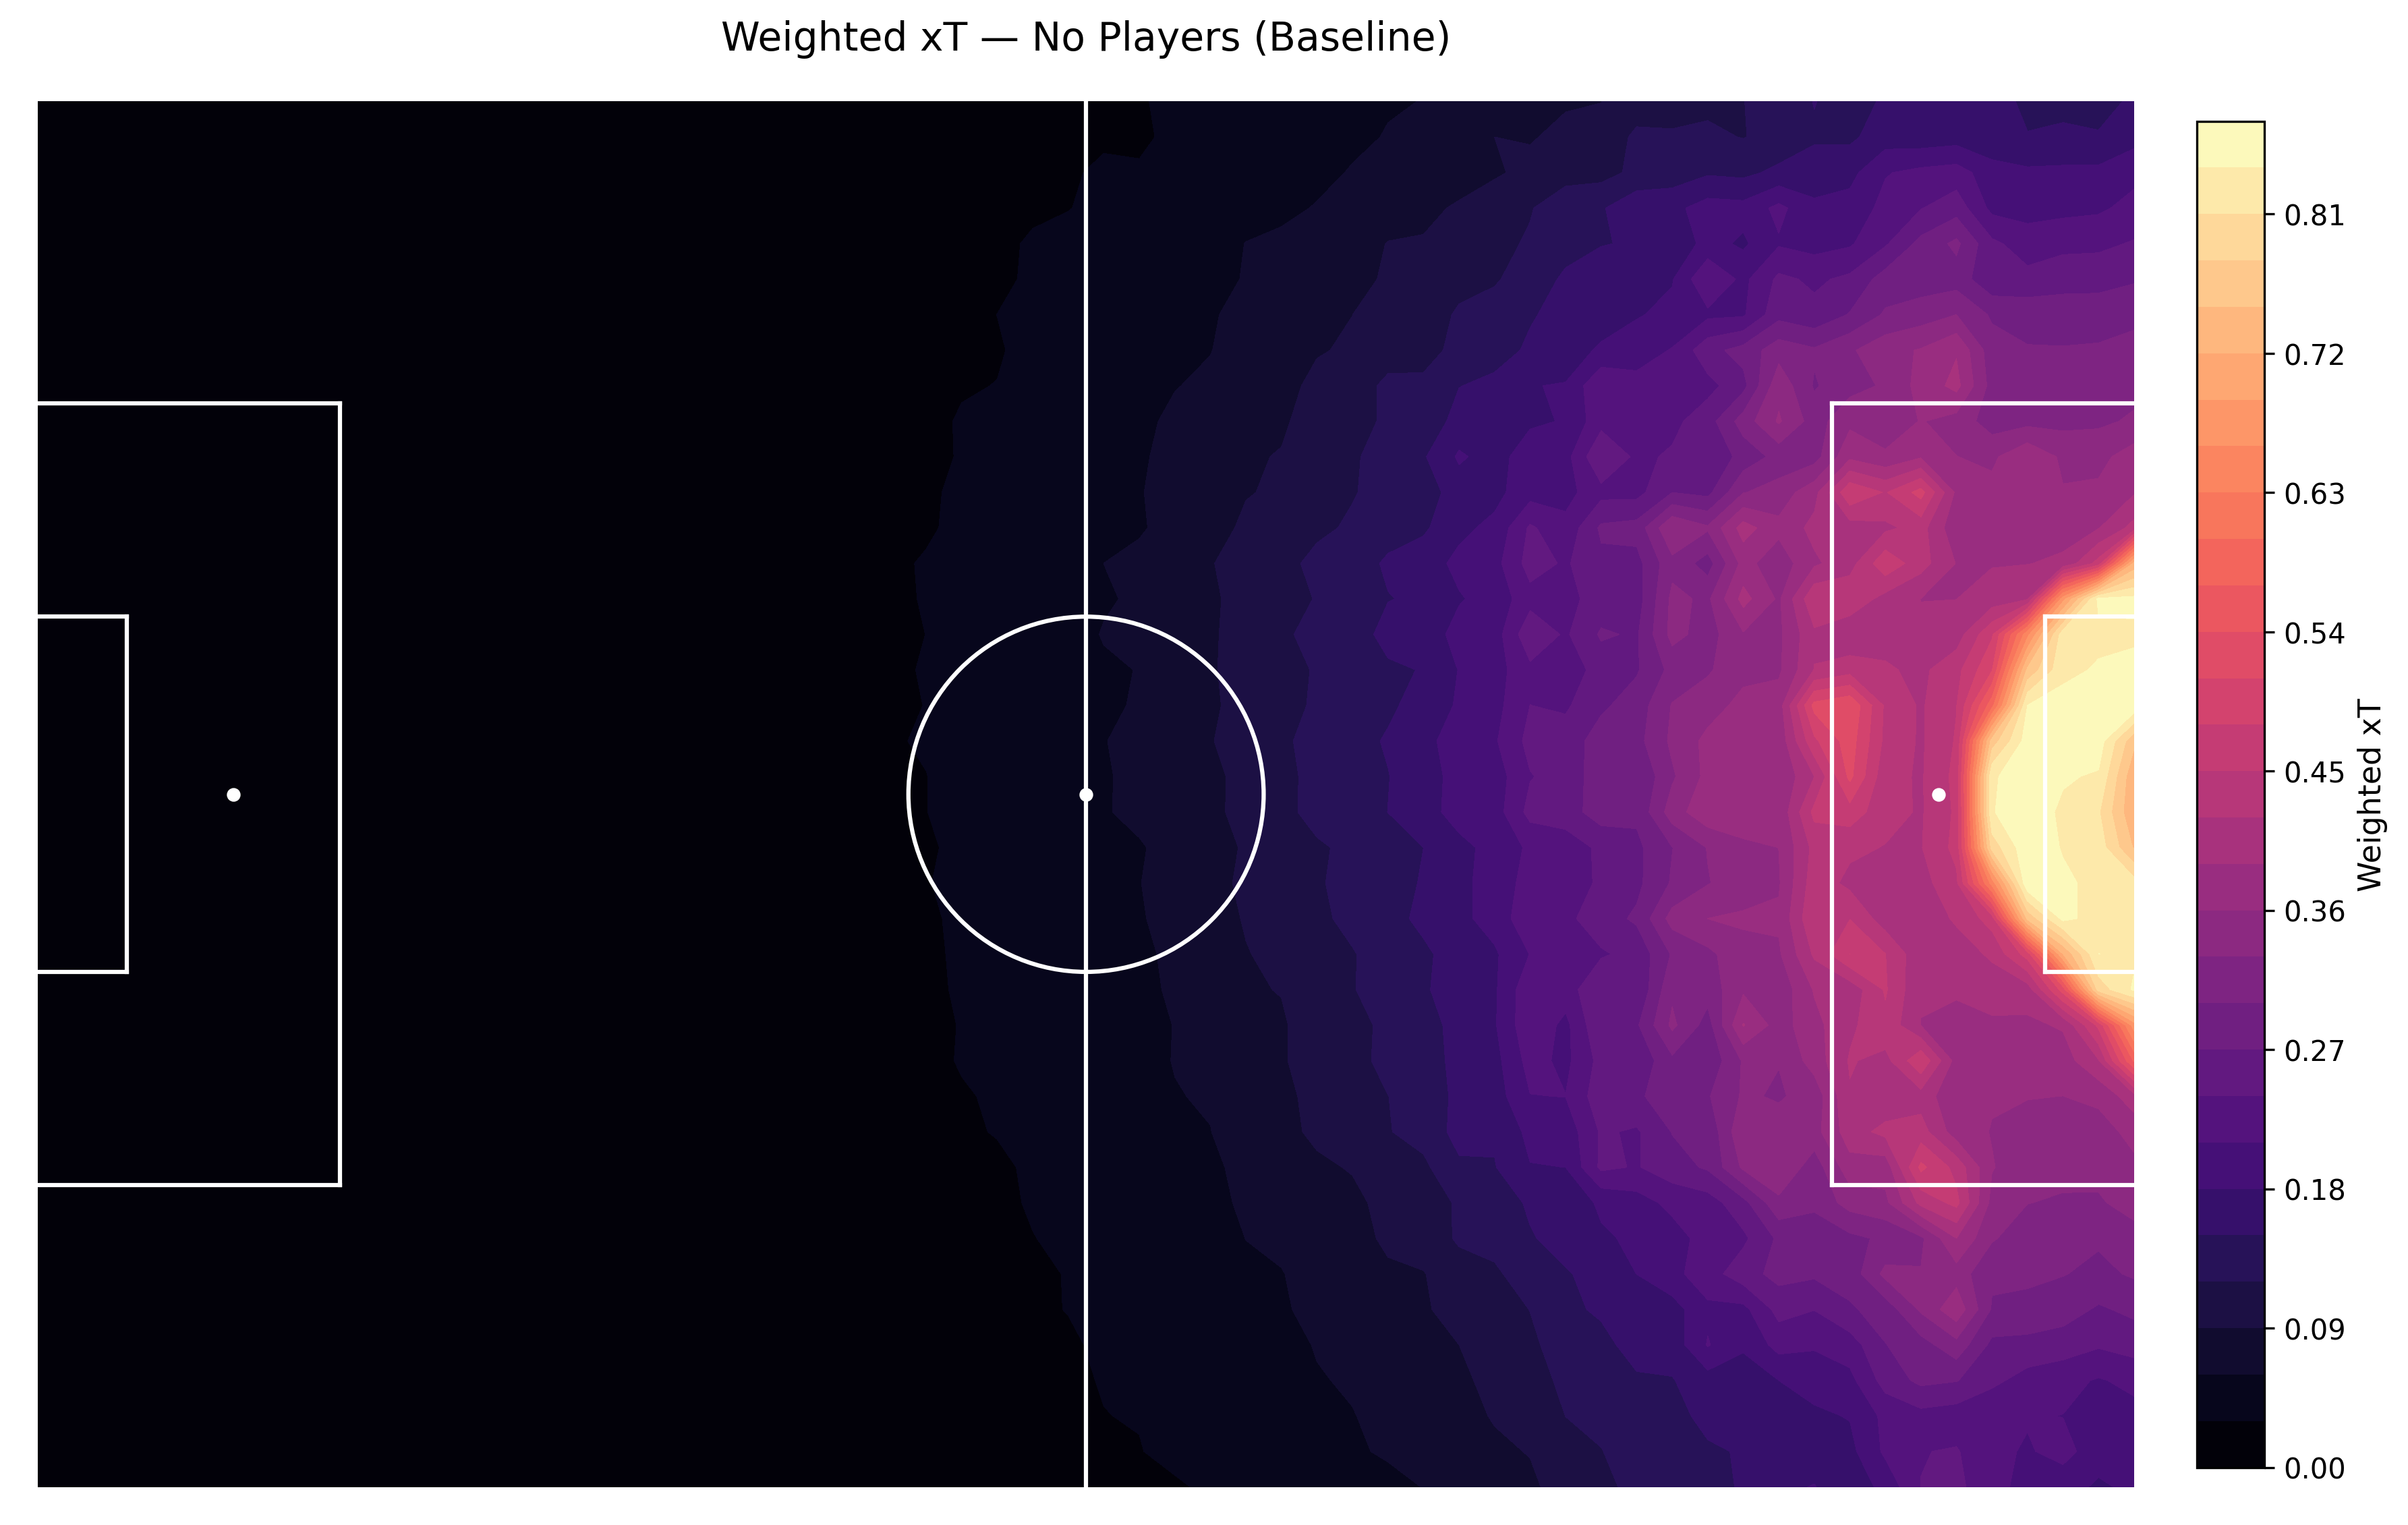
\includegraphics[width=0.8\textwidth]{xT_v3/xt_heatmap_weighted_v3.png}
    \caption{Non-Shot xT Heatmap: Version 3 Transformer, weighted action combination (no players, baseline). Threat peaks near the goal and is modulated by the action-type weighting inferred from player positions.}
\end{figure}

The Version 3 baseline heatmap is visually similar to Version 2: both use the same weighted action combination with no players present, producing a radially symmetric surface that peaks near goal. The key difference is in the texture of the threat surface. Version 2 is smoothly radial with clean contour rings, reflecting the CNN's tendency to produce well-behaved spatial gradients. Version 3 shows subtle ridges and irregular hot spots in the attacking third, the Transformer's contribution: even without explicit player tokens, Stage 2 has learned to apply small non-uniform adjustments to the Stage 1 baseline based on the spatial relationship between ball position and the implicit prior on where defenders are likely to be.

\begin{figure}[h]
    \centering
    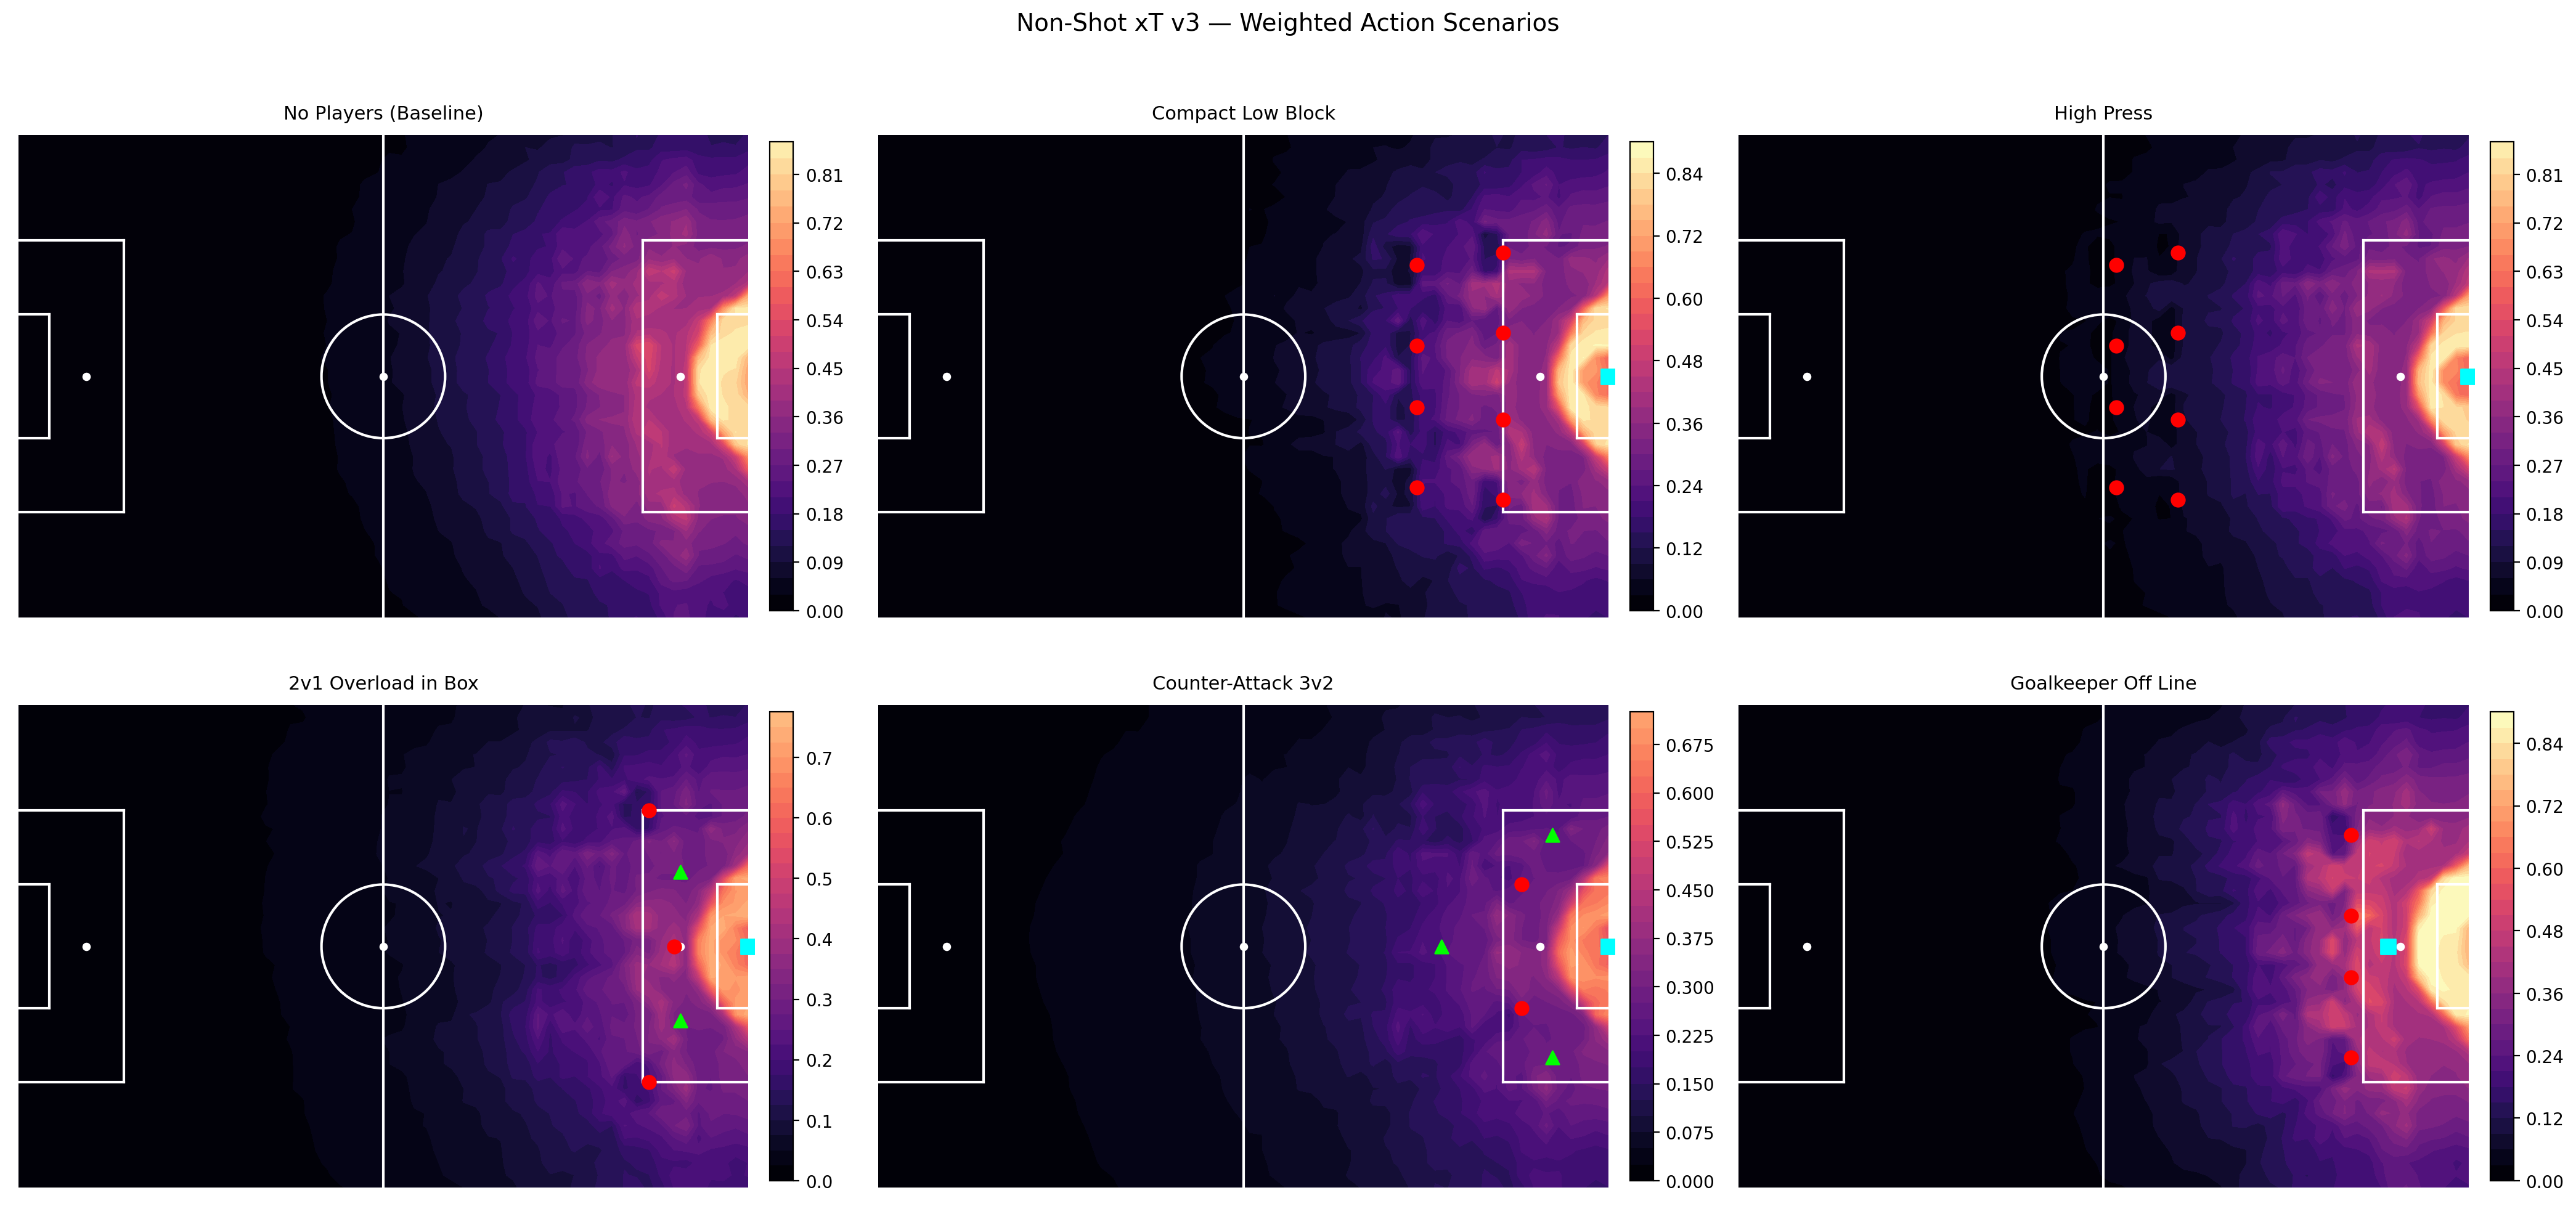
\includegraphics[width=0.8\textwidth]{xT_v3/xt_scenarios_weighted_v3.png}
    \caption{Scenario comparison: Version 3, weighted xT. Different defensive formations (Compact Low Block, High Press, 2v1 Overload, Counter-Attack 3v2, Goalkeeper Off Line) produce clearly different threat landscapes, demonstrating that Stage 2 is successfully modulating the positional baseline based on player context.}
\end{figure}

The six Version 3 scenario panels show considerably more differentiation than the equivalent Version 2 panels, and each produces a qualitatively distinct pattern that corresponds to the specific tactical configuration.

\textbf{No Players (Baseline).} The threat surface follows the same radial gradient as Version 2 but with visible texture: subtle ridges and hot spots appear in the attacking third, reflecting the Transformer's learned prior about where defenders are typically positioned even in the absence of explicit tokens.

\textbf{Compact Low Block.} With eight defenders forming two compact lines across the width of the box, the Version 3 heatmap shows a clearly suppressed central channel. Threat is not globally reduced; instead, it is redirected toward wider angles, reflecting that the Transformer has learned to associate a dense central defensive wall with diminished central threat while leaving wide approaches less affected. This selective suppression is absent from the Version 2 panel, which shows the same symmetric surface as the baseline.

\textbf{High Press.} Defenders positioned at $x = 62$--$72$ push far up the pitch. Version 3 responds by preserving threat near goal (correctly, since no defenders are close) but the Transformer also produces elevated values in the space behind the high line itself --- the model has learned that high-stationed defenders imply an exposed channel in the attacking half. This is a formation-level inference that Version 2 cannot make.

\textbf{2v1 Overload in Box.} Two attacking teammates at $(108, 28)$ and $(108, 52)$ create a numerical advantage over the lone central defender at $(107, 40)$. The Version 3 heatmap shows a pronounced amplified hot spot in the penalty area, noticeably larger and brighter than the baseline, concentrated near where the overloading runners are positioned. The wide covering defenders at $(103, 18)$ and $(103, 62)$ produce visible local suppression at the flanks, directing the peak threat inward toward the overload zone.

\textbf{Counter-Attack 3v2.} Three attackers are spread across wide and central positions ($(110, 22)$, $(110, 58)$, $(92, 40)$) with two defenders at $(105, 30)$ and $(105, 50)$. The Version 3 heatmap shows a bimodal threat distribution: elevated values in both wide channels, corresponding to the two advanced wide runners behind the defensive line, with a secondary cluster near the central link at $x = 92$. The two defenders create a corridor of reduced threat between them that separates the two bright flanks.

\textbf{Goalkeeper Off Line.} The keeper is placed at $x = 106$, leaving a clear gap between keeper and goal line. This is the most visually distinctive Version 3 panel: threat is markedly elevated directly at the goal mouth, immediately behind the keeper's position. The Transformer recognises that a keeper who has rushed off the line creates an open-goal opportunity that no other defensive shape produces. This panel has the highest global peak across all scenarios in either version.

\subsection{Cross-Version Scenario Comparison}

Comparing the two scenario grids side by side reveals what each architecture can and cannot represent.

\textbf{Formation sensitivity.} The most striking difference is the Compact Low Block vs High Press pair. In Version 2, both panels are essentially identical to the baseline: the CNN sees high defensive density in both cases and responds similarly regardless of where the defenders are positioned. In Version 3, these two scenarios produce opposite effects --- the Compact Low Block suppresses the central channel at goal, while the High Press leaves that area open and highlights the space behind the defensive line. This is a qualitative difference in what the model understands: Version 2 counts defenders; Version 3 reasons about their shape and location relative to the ball.

\textbf{Overload detection.} The 2v1 Overload in Box scenario shows a moderate amplification in Version 2 (driven by the Pass weight from two teammates) but a clearly pronounced and spatially concentrated hot spot in Version 3. The Transformer not only registers the numerical advantage but also concentrates the amplification near where the two attacking runners are positioned, rather than distributing it broadly.

\textbf{Open-goal recognition.} The Goalkeeper Off Line scenario is the clearest example of individual-player reasoning. Version 2 produces a very subtle change relative to its baseline; the keeper's Gaussian blob moves, but the CNN cannot extract a meaningful football inference from that. Version 3 correctly identifies the uncovered goal area and produces the highest threat values of any scenario, directly at the gap behind the keeper's position.

\textbf{What drives the difference.} The distinction is not simply that Version 3 is a better model: the two architectures are given identical information (same player positions) but process it fundamentally differently. Version 2 projects each player into a blurred density channel; the CNN's receptive field then perceives smooth local patterns in that density, which loses the identity of individual players and their specific spatial relationships. Version 3 encodes each player as a token and uses cross-attention to let the ball position query the player context explicitly, making formation shape, numerical balance, and individual player roles all directly accessible to the model.

% ============================================================
\section{Comparative Evaluation}\label{sec:comparison}
% ============================================================
% TODO: This is the academic heart of the cross-version standardisation work.
% Aim for 1--2 pages. Structure it as: table → metric-by-metric discussion →
% what drives each step change → overall conclusion on the progression.

\subsection{Results Summary}

% TODO: Fill in the v3 column once training is complete. The v1 and v2 values
% are confirmed from metrics_v1.json and metrics_v2.json respectively.
%
% v1: ROC AUC 0.6828 | Brier 0.0159 | Log Loss 0.0795 | Spearman 0.0810
% v2: ROC AUC 0.8416 | Brier 0.0067 | Log Loss 0.0413 | Spearman 0.0816
% v3: ROC AUC 0.8459 | Brier 0.0045 | Log Loss 0.0302 | Spearman 0.0843
%
% Note on comparability: v1 test set = all events from ~521 matches;
% v2/v3 test set = same 49 freeze-frame matches (140,697 events).
% The v1→v2 step therefore reflects both an architecture improvement AND
% a data upgrade (gaining player positions). The v2→v3 step is a pure
% architecture comparison on identical data.

\begin{table}[h]
\centering
\caption{Test set results across all three model versions. v1 is evaluated on all events; v2 and v3 are evaluated on the same 49 freeze-frame test matches for a direct comparison.}
\begin{tabular}{lcccc}
\toprule
\textbf{Model} & \textbf{ROC AUC} $\uparrow$ & \textbf{Brier} $\downarrow$ & \textbf{Log Loss} $\downarrow$ & \textbf{Spearman $\rho$} $\uparrow$ \\
\midrule
v1: Random Forest     & 0.6828 & 0.0159 & 0.0795 & 0.0810 \\
v2: CNN + MLP         & 0.8416 & 0.0067 & 0.0413 & 0.0816 \\
v3: Transformer       & 0.8459 & 0.0045 & 0.0302 & 0.0843 \\
\bottomrule
\end{tabular}
\label{tab:results}
\end{table}

\subsection{Discussion}

% TODO: Write 3--4 paragraphs interpreting the table above.
% Suggested structure:
%
% Paragraph 1 — v1 baseline:
%   The v1 ROC AUC of 0.659 shows the model can do better than random (0.5) but
%   is far from strong. The Spearman rho of 0.070 confirms the model learns a rough
%   positional ranking but is dominated by distance-to-goal. Refer back to feature
%   importance finding.
%
% Paragraph 2 — v1 → v2 step:
%   The jump to ROC AUC 0.842 (+18pp) and halving of both Brier and Log Loss
%   represents the largest single improvement. Discuss what drives it: (a) the CNN
%   architecture can learn non-linear spatial patterns that the RF cannot, (b) the
%   addition of full player positional context from 360 data. Note the caveat:
%   this step involves both an architecture change AND a data change, so the two
%   contributions cannot be fully separated.
%
% Paragraph 3 — v2 → v3 step:
%   The v2 → v3 comparison is a pure architecture comparison (same 49 test matches,
%   same events). Discuss the observed delta-rho from training and what it means.
%   If the improvement is small, discuss why: the CNN may already be capturing
%   most of the positional signal, the Transformer's residual adjustment has a
%   limited range, or the training set size (323 matches) may be insufficient
%   for the Transformer to learn subtle relational patterns.
%
% Paragraph 4 — overall:
%   The progression from v1 to v3 demonstrates that both richer data and more
%   expressive architectures contribute to improved xT modelling. The standardised
%   evaluation framework makes these improvements directly legible.
Version 1's ROC AUC of 0.6828 confirms that a Random Forest trained on tabular features can do better than random, but not by a large margin. The Spearman $\rho$ of 0.0810 reflects that the model learns a rough ordering: events closer to goal tend to score higher, dominated by distance and angle. The context features (\texttt{minute}, \texttt{score\_diff}, \texttt{team\_form}) each contribute a genuine share of around 6--8\% of total feature importance, collectively accounting for roughly 20\% of the model's predictive power, but the fundamental limit is the absence of player positional data. No scalar feature vector can encode the spatial arrangement of 22 players, and the binary labelling scheme does not reward actions that were close to generating a goal but did not quite get there.

The step from Version 1 to Version 2 produces the largest single improvement across every metric: ROC AUC increases by 16 percentage points (0.6828 $\to$ 0.8416), Brier Score more than halves (0.0159 $\to$ 0.0067), and Log Loss nearly halves too (0.0795 $\to$ 0.0413). Two things change simultaneously at this step: the architecture moves from a Random Forest to a dual-branch CNN, and the training data gains full player positional context from the 360 freeze-frame data. It is not possible to fully separate the contribution of each, but together they represent a substantial upgrade in both the richness of the input and the model's capacity to learn from it.

The step from Version 2 to Version 3 is a pure architecture comparison on identical data, and the results are more modest. ROC AUC improves marginally (0.8416 $\to$ 0.8459), while Brier and Log Loss improve more noticeably (0.0067 $\to$ 0.0045 and 0.0413 $\to$ 0.0302). However, Spearman $\rho$ barely changes (0.0816 $\to$ 0.0843), and during training the per-epoch $\Delta\rho$ relative to the Stage 1 CNN baseline was consistently around $-0.0002$, indicating the Transformer cross-attention did not meaningfully improve rank ordering above what the CNN alone had already learned. The improvements in Brier and Log Loss suggest the Transformer is refining the calibration of the probability values without changing how events are ranked. This may be because the CNN's spatial representation already captures most of the positional signal available in 323 matches, leaving limited room for the Transformer's relational reasoning to contribute.

Overall, the progression from Version 1 to Version 3 demonstrates that both richer data and more expressive architectures contribute to improved xT modelling. The two biggest gains came from introducing player positional context (the 360 data) and adopting a deep learning architecture capable of learning non-linear spatial patterns. The standardised four-metric evaluation framework makes these improvements directly comparable across all three versions.

\subsection{Limitations and Threats to Validity}

% TODO: Discuss potential threats to the validity of the comparison:
%   1. The v1/v2 test scopes differ (all events vs freeze-frame only) --- explain
%      why this is a deliberate design choice and what it means for interpretation
%   2. The small freeze-frame dataset (323 matches, 49 test) means v2/v3 results
%      may have higher variance than v1
%   3. Spearman rho is sensitive to the label distribution; the discounted soft
%      labels in v2/v3 are themselves an approximation of true contribution
%   4. All models trained on a single random seed --- results may vary with different splits
There are four threats to the validity of the cross-version comparison that are worth acknowledging.

First, the Version 1 and Version 2/3 test sets are not the same population of events. Version 1 is evaluated on all events from 520 matches, while Versions 2 and 3 are evaluated on 140,697 events from 49 freeze-frame matches. This is a deliberate design choice that reflects the data actually available to each model, but it means the Version 1 $\to$ Version 2 improvement cannot be attributed to architecture alone. Some of the gain may come from the fact that freeze-frame matches are, by nature, a curated subset of the dataset.

Second, the freeze-frame dataset is considerably smaller than the full event dataset (323 matches versus 3,464), so the Version 2 and Version 3 test results are based on fewer matches. With only 49 test matches, the metric estimates may have higher variance than the Version 1 results, and a different random seed could produce a noticeably different test set.

Third, the Spearman $\rho$ values for Versions 2 and 3 are computed against soft discounted labels, which are themselves an approximation of each event's true contribution to a goal. The $\gamma = 0.9$ discount factor is a modelling assumption, not ground truth, and a different choice of $\gamma$ would produce different label distributions and different $\rho$ values.

Finally, all three models were trained and evaluated using a single random seed (42). Results may vary under different splits, and it is possible that the Version 3 $\Delta\rho$ would be more positive or negative under a different partition of the 323 freeze-frame matches.

% ============================================================
\section{Visualisations and Frontend}\label{sec:viz}
% ============================================================

With a trained model in hand, it is important to present the predictions in a form that is intuitive for football analysts and fans. Two visualisation approaches were developed.

\subsection{xT Heatmap}

For each version of the model, a heatmap of the predicted xT value across the entire pitch is generated. The pitch is divided into a grid and the model is queried at each grid cell, sweeping the ball position across all positions. The resulting probability values are plotted as a filled contour plot using the \texttt{magma} colourmap (dark/purple = low threat, orange/bright = high threat), with standard pitch markings overlaid in white for reference.

For Version 1, a single heatmap is produced using a Pass action type. For Versions 2 and 3, a \textbf{weighted action combination} is used: for each grid cell, the model is run for all four action types (Shot, Pass, Carry, Dribble), and the results are combined using action weights inferred from player positions. This produces a single heatmap representing the overall threat value of having the ball at each position, accounting for what action is most likely to be taken. The weight formulas are identical across Versions 2 and 3 and the frontend: Shot weight decreases with distance and blocked shooting lanes; Pass weight increases with available outfield teammates (up to 5); Carry weight decreases with nearby defenders; Dribble weight increases when defenders are pressing close. For Pass actions, the model is run once per outfield teammate and the maximum xT across all targets is taken, mirroring the frontend behaviour.

In addition, a \textbf{scenario comparison} grid is generated for Versions 2 and 3, showing how different defensive formations affect the threat landscape. The scenarios tested include:
\begin{itemize}
    \item No players (baseline positional threat)
    \item Compact Low Block (defenders packed in front of goal)
    \item High Press (defenders pushed high into the opponent's half)
    \item 2v1 Overload in Box (two attackers vs one defender in the penalty area)
    \item Counter-Attack 3v2 (three attackers vs two covering defenders)
    \item Goalkeeper Off Line (goalkeeper rushed out to the edge of the box)
\end{itemize}

\subsection{Interactive Web Frontend}

To make the Version 3 model accessible and easy to explore, a Flask-based interactive web application was developed. The frontend renders a football pitch as an HTML5 canvas, and allows the user to:

\begin{itemize}
    \item Click to place the ball start position
    \item Place outfield teammates, outfield opponents, a friendly goalkeeper, and an opponent goalkeeper using mode buttons
    \item Click ``Predict'' to query the model in real time
\end{itemize}

The Flask backend receives the ball and player positions as a JSON payload. Rather than requiring the user to specify an action type, the backend \textbf{infers the action context automatically from the player positions}: the Shot weight increases as the ball approaches goal and the shooting lane is clear; Pass weight increases with the number of outfield teammates available; Carry weight decreases with the number of defenders close by; and Dribble weight increases when defenders are pressing nearby. The weighted xT is computed as $\sum_a P(\text{action}=a) \times \text{xT}(a)$, and the breakdown by action type is returned alongside the headline figure.

The result is displayed as a large ``xT'' value, with a breakdown table showing each action's weight, individual xT, and contribution to the weighted total. This allows users to understand not just what the model's overall assessment is, but \textit{why} : which action types are driving the prediction for that ball position and player layout.

\begin{figure}[h]
    \centering
    % TODO: Replace with actual screenshot — run `python3 xtv3fe/app.py`, open
    % http://localhost:5000 in a browser, place some players, and save a screenshot
    % as frontend_screenshot.png in the project root.
    \fbox{\parbox{0.85\textwidth}{\centering\vspace{2cm}
    \textit{[Screenshot of the interactive xT web frontend to be inserted here.\\
    Run \texttt{python3 xtv3fe/app.py} and capture the browser window.]}
    \vspace{2cm}}}
    \caption{Interactive xT web frontend: the user places players on the pitch and
             the model returns a real-time weighted xT prediction with per-action breakdown.}
\end{figure}

% ============================================================
\section{Conclusion}\label{sec:conclusion}
% ============================================================

This project has developed a Non-Shot Expected Goals model that progresses through three increasingly sophisticated architectures, each addressing the key limitations of the previous version.

Version 1 established a working baseline using a Random Forest on positional and context features (including match score, period, elapsed minute, and team form). While functional, it confirmed the known limitation of this approach: the model is dominated by a distance-to-goal heuristic, and even with context features the absence of player positional data prevents it from capturing the richer spatial dynamics of a possession sequence.

Version 2 addressed this by moving to a dual-branch CNN architecture trained on StatsBomb 360 data, encoding the full pitch as a multi-channel spatial image. This allowed the model to see where all players are, not just the ball, and to reason about the spatial patterns of play. With 1,036,140 events from 323 matches, the model achieved a test ROC AUC of 0.8416, a substantial improvement over Version 1, but the CNN's implicit spatial encoding still limits its ability to reason explicitly about individual player relationships.

Version 3 addressed this final limitation by adding a Transformer cross-attention layer on top of the frozen Version 2 CNN. Each player is now treated as an individual token, and the ball position queries the player context via attention, enabling explicit relational reasoning about who is where relative to the ball and goal. The resulting scenario heatmaps demonstrate qualitatively that the model correctly adjusts threat based on defensive formations in a way that Version 2 cannot.

The accompanying interactive frontend brings the model to life for a non-technical audience, allowing users to explore how different player arrangements affect xT in real time.

\textbf{Limitations and Future Work:}
\begin{itemize}
    \item The 360 data is available for only a subset of matches and competitions, limiting the training set for Versions 2 and 3.
    \item The class imbalance (goal rate $\approx 0.32\%$) makes training and evaluation challenging; more sophisticated imbalance handling (e.g.\ focal loss) could improve calibration.
    \item Player identity and movement trajectories are not used; the model sees only a static snapshot. Incorporating sequential information (e.g.\ via an LSTM or temporal attention) could further improve predictions.
    \item A more principled action-weight inference (e.g.\ trained jointly with the xT model) would improve the quality of the weighted visualisations.
\end{itemize}

Overall, the project demonstrates a clear progression from a simple machine learning baseline to a sophisticated deep learning model capable of contextualising attacking threat in football with player-level spatial reasoning.

% ============================================================
% REFERENCES
% ============================================================
% TODO: Replace each \bibitem below with proper bibliographic details.
% Aim for at least 10 references. Suggested sources are listed in the comments.
% Use a consistent citation style (Harvard or IEEE are most common for CS FYPs ---
% check your department's requirements).

\begin{thebibliography}{99}

\bibitem{reep1968}
Reep, C. and Benjamin, B., 1968. Skill and chance in association football. \textit{Journal of the Royal Statistical Society. Series A (General)}, 131(4), pp.\ 581--585.

\bibitem{statsbomb2018}
StatsBomb, 2018. \textit{StatsBomb Open Data} [online]. Available at: \url{https://github.com/statsbomb/open-data} [Accessed: 28 April 2026].

\bibitem{singh2019}
Singh, K., 2019. \textit{Introducing Expected Threat} [blog post]. Available at: \url{https://karun.in/blog/expected-threat.html} [Accessed: 28 April 2026].

\bibitem{decroos2019}
Decroos, T., Bransen, L., Van Haaren, J. and Davis, J., 2019. Actions speak louder than goals: Valuing player actions in football. In: \textit{Proceedings of the 25th ACM SIGKDD International Conference on Knowledge Discovery \& Data Mining}, pp.\ 2249--2258.

\bibitem{pappalardo2019}
Pappalardo, L., Cintia, P., Rossi, A., Massucco, E., Ferragina, P., Pedreschi, D. and Giannotti, F., 2019. A public data set of spatio-temporal match events in soccer leagues. \textit{Nature Scientific Data}, 6, p.\ 236.

\bibitem{lecun1998}
LeCun, Y., Bottou, L., Bengio, Y. and Haffner, P., 1998. Gradient-based learning applied to document recognition. \textit{Proceedings of the IEEE}, 86(11), pp.\ 2278--2324.

\bibitem{vaswani2017}
Vaswani, A., Shazeer, N., Parmar, N., Uszkoreit, J., Jones, L., Gomez, A.N., Kaiser, \L. and Polosukhin, I., 2017. Attention is all you need. In: \textit{Advances in Neural Information Processing Systems}, 30.

\bibitem{devlin2019}
Devlin, J., Chang, M., Lee, K. and Toutanova, K., 2019. BERT: Pre-training of deep bidirectional transformers for language understanding. In: \textit{Proceedings of NAACL-HLT 2019}, pp.\ 4171--4186.

\bibitem{breiman2001}
Breiman, L., 2001. Random forests. \textit{Machine Learning}, 45(1), pp.\ 5--32.

\bibitem{statsbomb360}
StatsBomb, 2020. \textit{StatsBomb 360 Data} [online]. Available at: \url{https://statsbomb.com/articles/soccer/statsbomb-360-freeze-frame-data-a-brief-guide/} [Accessed: 28 April 2026].

\bibitem{statsbombpy}
StatsBomb, 2020. \textit{StatsBombPy} [software]. Available at: \url{https://github.com/statsbomb/statsbombpy} [Accessed: 28 April 2026].

\end{thebibliography}

% ============================================================
% APPENDICES
% ============================================================

\begin{appendices}

\section{Code Structure}

The full source code for all three versions is available in the project repository. The key files are:

\begin{itemize}
    \item \textbf{Version 1} (\texttt{xT\_v1/}): \texttt{parser.py}, \texttt{builder.py}, \texttt{loader.py}, \texttt{model.py}: data extraction, chaining, and Random Forest training.
    \item \textbf{Version 2} (\texttt{xT\_v2/}): \texttt{config.py}, \texttt{encoder.py}, \texttt{builder.py}, \texttt{dataset.py}, \texttt{model.py}, \texttt{train.py}, \texttt{visualize.py}: full CNN pipeline with 360 data.
    \item \textbf{Version 3} (\texttt{xT\_v3/}): \texttt{config.py}, \texttt{builder.py}, \texttt{dataset.py}, \texttt{model.py}, \texttt{train.py}, \texttt{visualize.py}: two-stage Transformer pipeline.
    \item \textbf{Frontend} (\texttt{xtv3fe/}): \texttt{app.py}, \texttt{templates/index.html}: Flask interactive web application.
    \item \textbf{Shared} (root): \texttt{evaluate.py}: standardised evaluation module used by all three versions.
\end{itemize}

Each version can be run end-to-end using the \texttt{main.py} entry point with \texttt{--build}, \texttt{--train}, and \texttt{--visualize} flags.

\section{Full Metric Tables}

\begin{table}[h]
\centering
\caption{Test set evaluation metrics across all three model versions.}
\begin{tabular}{lcccc}
\toprule
\textbf{Model} & \textbf{ROC AUC} $\uparrow$ & \textbf{Brier} $\downarrow$ & \textbf{Log Loss} $\downarrow$ & \textbf{Spearman $\rho$} $\uparrow$ \\
\midrule
v1: Random Forest  & 0.6828 & 0.0159 & 0.0795 & 0.0810 \\
v2: CNN + MLP      & 0.8416 & 0.0067 & 0.0413 & 0.0816 \\
v3: Transformer    & 0.8459 & 0.0045 & 0.0302 & 0.0843 \\
\bottomrule
\end{tabular}
\label{tab:metrics_full}
\end{table}

\begin{table}[h]
\centering
\caption{Dataset statistics and train/val/test split by model version.}
\begin{tabular}{lrrrrr}
\toprule
\textbf{Version} & \textbf{Matches} & \textbf{Total Events} & \textbf{Train Events} & \textbf{Val Events} & \textbf{Test Events} \\
\midrule
v1 (all events)      & 3,464 & 6,108,353 & 4,284,580 & 913,800 & 909,973 \\
v2/v3 (freeze-frame) & 323   & 915,139   & 637,926   & 136,516 & 140,697 \\
\bottomrule
\end{tabular}
\label{tab:dataset_stats}
\end{table}

\begin{table}[h]
\centering
\caption{Key hyperparameters for each model version.}
\begin{tabular}{llll}
\toprule
\textbf{Hyperparameter} & \textbf{v1 (RF)} & \textbf{v2 (CNN)} & \textbf{v3 (Transformer)} \\
\midrule
Architecture        & Random Forest       & Dual-branch CNN+MLP  & Frozen v2 + Transformer \\
Estimators / Epochs & 100 trees           & 50 epochs            & 40 epochs \\
Max depth / LR      & 12                  & $10^{-3}$            & $5{\times}10^{-4}$ \\
Weight decay        & N/A                 & $10^{-4}$            & $10^{-4}$ \\
Input features      & 10 scalar           & 6-ch image + 22 scalar & 6-ch image + 22 scalar + player tokens \\
Trainable params    & N/A                 & 1,282,369            & 121,601 \\
Train split seed    & 42                  & 42                   & 42 \\
Label type          & Binary              & Soft ($\gamma=0.9$)  & Soft ($\gamma=0.9$) \\
\bottomrule
\end{tabular}
\label{tab:hyperparams}
\end{table}

\end{appendices}

\end{document}
